\chapter{Scheduling with Communication Delays on Related Machines}\label{chapter: S2}

  \section{Introduction}
  We consider the problem of scheduling jobs with precedence and communication delay constraints on {\em related machines.}
  This classic model  was first introduced by Rayward-Smith~\cite{RAYWARDSMITH1987} and Papadimitriou and Yannakakis~\cite{PapadimitriouY90}.
  In this problem we are given a set  $J$ of $n$ jobs, where each job $j$ has a processing length $p_j  \in \setZ_+$ and a weight $w_j \in \setZ_+$.
  The jobs need to be scheduled on $m$ related machines, where machine $i \in [m]$ has speed $s_i  \in \setZ_+$.
  If a job $j$ with processing length $p_j$ is scheduled on the machine $i$, then it requires  $p_j/s_i$ time units to complete.
  In addition, we are  given a {\em communication delay parameter} $c \in  \setZ_{\ge 0}$.
  The jobs have precedence and communication delay constraints, which are given by a partial order $\prec$. 
  A constraint $j \prec j'$ encodes that job $j'$ can only start after job $j$ is completed.
  Moreover, if $j \prec j'$ and $j$, $j'$ are scheduled on {different machines}, then $j'$ can only start executing at least $c$ time units after $j$ had finished. 
  On the other hand,  if $j$ and $j'$ are scheduled on the {same machine}, then $j'$ can start executing immediately after $j$ finishes. 
  The goal is to schedule jobs {\em non-preemptively} so as to minimize a certain objective function.
  In a non-preemptive schedule, each job $j$ needs to be  assigned to a single machine $i$ and executed during a contiguous time interval of length $p_j/s_i$.
  
  \medskip
  We focus on two widely studied objective functions: (1) minimizing the weighted sum of completion times of jobs, and (2) minimizing the makespan.
  In the standard 3-field notation\footnote{
  We adopt the convention of \cite{GLLR79,VeltmanLL90}, where the respective fields denote:
      \textbf{(1) machine environment:} $Q$ for related machines, $P$ for identical machines,
      \textbf{(2) job properties:} $\Prec$ for precedence constraints; $c$ for communication delays of length $c$; $p_j = 1$ for unit length case,
      \textbf{(3) objective:} $\Cmax$ for minimizing makespan, $\wjcj$ for minimizing weighted sum of completion times.
  },
  these problems are denoted by $Q \mid \Prec, c \mid \wjcj$ and $Q  \mid \Prec, c \mid \Cmax$, respectively.
  In the presence of precedence and communication delay constraints, the weighted completion time objective is more general than the makespan, in the sense that one can use an approximation algorithm for the completion time objective to obtain a comparable result for the makespan.
  Our main motivation to study these problems is twofold:
  \begin{itemize}
  \item The problems of scheduling jobs with communication delays are some of the most notorious open questions in approximation algorithms and scheduling theory, which have resisted progress for a long time.  For this reason, the well-known survey by  Schuurman and Woeginger~\cite{SW99a} and its recent update by Bansal~\cite{Bansalmapsp} list understanding the approximability of the problems in this model as one of the top-10 open questions in scheduling theory.
  \item These problems arise in many real-world applications,  especially in the context of scheduling in data centers.
  A precedence constraint $j \prec j'$ typically implies that the input to $j'$ depends on the output of $j$.
  Hence, if $j$ and $j'$ are scheduled on different machines, then the {\em communication delay} due to transferring this output to the other machine often becomes the bottleneck.
  The problem has received significant attention in applied data center scheduling literature; see ~\cite{Chowdhury, guo2012spotting,hong2012finishing,shymyrbay2018meeting,zhang2012optimizing,zhao2015rapier,luo2016towards} for more details.
   Another timely  example is in the parallelization of Deep Neural Network training. When DNNs are trained on multiple clusters, the communication costs incurred for synchronizing the weight updates in fact dominate the overall execution time~\cite{narayanan2018pipedream}.
  The resulting \emph{device placement} problem~\cite{dean2017rlplacement,spotlight2018,jia2018beyond,tarnawski2020efficient}  is indeed a variant of scheduling with communication delays.
  \end{itemize}
  
  
  \medskip
  Scheduling jobs with precedence and communication delays has been studied extensively over many years \cite{RAYWARDSMITH1987,PapadimitriouY90,MunierKonig,HanenMunier73Apx,ThurimellaYesha,HoogeveenLV94,PapadimitriouY90,GiroudeauKMP08}.
  Yet,  very little was known in terms of the approximation algorithms for problem until the recent work by Maiti et al.~\cite{MRSSV} and us~\cite{DKRTZ20}.
  Previously, even for the {\em identical machines} case, where all machines have the same speed, the best algorithm for general~$c$  achieved an approximation factor of $2/3 \cdot (c+1)$~\cite{GiroudeauKMP08}, which only marginally improves on Graham's list scheduling algorithm that obtains a $(c+1)$-approximation, while requiring the assumption that $p_j = 1$.
  Moreover, no results were known for the related machines case.
  
  \medskip
  In a very recent work, we  \cite{DKRTZ20} designed an $O(\log m \log c)$-approximation algorithm for minimizing makespan in the {\em identical machines case.}
  We also showed an $O(\log n \log c)$-approximation algorithm for the weighted sum of completion times objective, in a special case where $p_j = 1$ and we have an {\em unlimited} number of machines. 
  In a parallel and independent work, Maiti {et al.}~\cite{MRSSV} developed an $O(\log^2 n \log^2 m \log c / \log \log n)$-approximation algorithm for the makespan objective function on {\em related machines}.
  Interestingly, these two results were obtained using rather different techniques.
  
  
  
  Maiti {et al.}~\cite{MRSSV} obtain a polylogarithmic approximation algorithm for scheduling in the presence of precedence and communication delay constraints in the {\em job duplication} model. 
  Here, a single job can be scheduled on {\em multiple machines}, which is known to effectively ``hide'' the communication delay constraints \cite{PapadimitriouY90}.
  Quite surprisingly, Maiti {et al.} then show that one can convert a schedule with duplication to a feasible schedule without duplication, 
  where every job is processed on a single machine, while increasing the makespan by at most an $O(\log^2 n \log m)$ factor.
  To create a strict contrast between our techniques and that of Maiti {et al.}, 
  we do not consider the duplication setting or any reduction from it.
  Additionally, the LP of Maiti {et al.} does not give rise to a {\em semimetric} on the set of jobs, 
  which is a crucial part of our scheduling algorithm.
  
  The framework of Maiti {et al.} extends to the weighted sum of completion times objective, but it obtains 
  an extra additive term in the approximation that may dominate the factor; 
  we discuss this further in Section~\ref{sec:challenges}.
  Moreover, our previous results~\cite{DKRTZ20} also do not imply any approximation guarantees for the related machines case.
  Specifically, in the presence of communication delay constraints there are no known reductions
  between the sum of weighted completion time and makespan objective functions similar to~\cite{UniformlyRelatedMachinesWithPrecedences-ChudakShmoys-JALG99}.
  
  Finally, in another recent work, Su et al.~\cite{weirman} studied the objective of minimizing makespan and sum of weighted completion times on related machines. 
  They showed that a Generalized Earliest Time First (GETF) algorithm achieves a makespan of $O(\log m/\log \log m) \cdot OPT + C$, where $C$ is the total communication delay in the longest chain in the input graph.
  They show a similar bound on the schedule produced by GETF for the weighted sum of completion times objective.
  However, both of these bounds do not give any multiplicative approximation guarantees, as the additive terms can be substantially higher than the optimal solution.
  The additive terms in above bounds are precisely the reason why the scheduling with communication delays problem is significantly more challenging than the case when $c = 0$.
  
  
  
  
  \subsection{Our Contributions}
  
  Let $M$ denote the number of machines types or equivalently speed classes.
  By standard arguments we can assume that $M =\log(s_{\text{max}}/s_{\text{min}})\leq O(\log m)$ while only losing a constant factor in the approximation guarantee, where $s_{\text{max}}$ and $s_{\text{min}}$ denote the fastest and slowest speeds of machines in the input instance.
  
  The main result of this paper is the following:
  
  \begin{theorem} \label{thm:main}
  There is a randomized $O(M^2 \cdot \log^2 n)$-approximation algorithm for $Q \mid \Prec, c \mid \sum_{j} w_j C_j$ with expected polynomial running time. When jobs have unit processing lengths, $Q \mid \Prec, c, p_j = 1 \mid \sum_{j} w_j C_j$, the approximation factor of the algorithm improves to  $O(M \cdot \log^2 n )$.
  \end{theorem}
  
  As $M \leq O(\log n)$, our result gives an  $O(\log^4 n)$-approximation algorithm to the general problem and an $O(\log^3 n)$-approximation algorithm for the case with unit processing lengths.
  As a byproduct of our result we also obtain an improved approximation for the makespan objective function.
  
  
  \begin{theorem} \label{thm:colmain}
  There is a randomized $O(M \cdot \log m \cdot \log n)$-approximation algorithm for $Q \mid \Prec, c \mid \Cmax$ with expected polynomial running time. When jobs have unit processing lengths, $Q \mid \Prec, c, p_j = 1 \mid \Cmax$, the approximation factor of the algorithm improves to  $O(\log m \cdot \log n)$.
  \end{theorem}
  
  So our result gives an $O(\log^3 n)$-approximation algorithm for the problem of minimizing makespan (and an $O(\log^2 n)$-approximation algorithm for the case with unit processing lengths). 
  This improves the $O(\log^5 n / \log \log n)$-approximation algorithm due to Maiti {et al.}~\cite{MRSSV}.
  
  
  \subsection{Technical Challenges}
  \label{sec:challenges}
  Absent the communication delay constraints, one can use an approximation for the makespan objective to obtain an approximation algorithm for the weighted sum of completion times objective, with some (negligible) loss in the approximation quality \cite{hall1997scheduling,queyranne2002approximation,li2020scheduling}.
  Namely, a standard approach is to first solve an LP for the weighted sum of completion times problem, and then geometrically partition jobs according to completion times  in the LP solution
  into buckets of the form $[2^t, 2^{t+1}]$.
  Next, use an $\alpha$-approximation algorithm for makespan to schedule these jobs in an interval of length $O(\alpha \cdot 2^t)$.
  Finally, concatenate the schedules of jobs belonging to different partitions.
  This approach gives an $O(\alpha)$-approximation for identical machines, and an extension of this idea to related machines is given by \cite{UniformlyRelatedMachinesWithPrecedences-ChudakShmoys-JALG99}.
  
  However, this approach fails in the presence of communication delay constraints, even for the identical machines case.
  In particular, the main technical difficulty arises when in the LP solution a large number of jobs have very small completion times, say $O(c/\log^2 n)$.
  We need to schedule these jobs so that no precedence and communication delay constraints are violated, while at the same time achieving completion times comparable to the LP.
  This requires very precise control over job completion times, which cannot be achieved by the existing algorithms for the makespan.
  The problem becomes further more complex if machines have different speeds and jobs have different weights.
  This is also the main technical hurdle if one tries to adapt the framework of Maiti {et al.}~\cite{MRSSV}.
  In fact,  \cite{MRSSV} gives a schedule whose cost can be as large as $O\left ((\log^5 n/\log \log n) \cdot OPT + c \cdot \sum_{j} w_j \right)$, which only implies an approximation factor of $\max \{c, \log^5 n/\log \log n \}$.
  
  
  
  \subsection{Our Techniques and Algorithm Overview}
  
  We obtain our results by generalizing the LP hierarchy framework introduced by \cite{DKRTZ20} to handle processors of varying speed and the more general objective of minimizing the weighted sum of completion times. In this section we outline our main techniques and explain our innovations compared to \cite{DKRTZ20}. In particular, as alluded above, the weighted sum of completion times objective requires a finer control over the {\em time slots where jobs are scheduled} compared to minimizing the makespan. Moreover, allowing different machine types introduces an {\em assignment} aspect to the problem, namely assigning jobs to a machine type, which is not present in the identical machines case.
  Tackling these two challenges simultaneously requires an extended LP as well as more structural insights about the solution produced by the Sherali-Adams hierarchy compared to \cite{DKRTZ20}. 
  
  \medskip
  To keep the notation simple we will use $\log n$ instead of the potentially smaller quantities $\log m$ and $M$. 
  We begin our discussion with the problem $\mathsf{Q} \mid \mathsf{prec}, p_j=1, c \mid \sum w_jC_j$, where jobs have unit lengths. 
  We will see later that we can reduce the version with general processing times to the case $p_j=1$ while losing a factor of $O(\log n)$. A helpful view that already emerged in preceeding work is to partitition the time horizon into intervals of length $c$ or larger. Then if one can assign each job $j_1$ so that any predecessor $j_2$ is either executed on the same machine or in a earlier interval, then inserting a waiting time of $c$ after each interval will result in a valid schedule while completion times increase by at most a factor of 2.
  
  We start by designing an LP with \emph{time-indexed variables} $x_{j,i,t}$ that specify whether job $j$ is to be scheduled in time slot $t$ on machine $i$. To accommodate the different speeds, a machine in class $k$ has $s_k$ slots available per unit time interval. Similarly to \cite{DKRTZ20}, we take the \emph{Sherali-Adams lift} with a constant number of rounds and use it to extract variables $y_{j_1,j_2}$, which tell us whether the jobs are scheduled on the same machine within an interval of length $c$, as well as variables $C_j$, which denote the \emph{LP completion times}. Our main LP rounding result is that we can generate a schedule at random so that the completion time of every job is at most $O(\log^3 n) \cdot C_j$ in expectation.
  
  Using the Sherali-Adams properties one can prove that the function $d : J \times J \to \setR_{\geq 0}$ with $d(j_1,j_2) := 1- y_{j_1,j_2}$ is a \emph{semimetric}. One important ingredient of our algorithm is a clustering procedure due to Calinescu, Karloff and Rabani~\cite{DBLP:journals/siamcomp/CalinescuKR04} which, for such a semimetric space $(J,d)$ and a parameter $\Delta>0$, finds a random partition $J = V_1 \dot{\cup} \ldots \dot{\cup} V_q$ into blocks of diameter at most~$\Delta$ such that any set $U \subseteq J$ has a probability of at most $O(\log(n) \cdot \frac{\textrm{diam}(U)}{\Delta})$ of being separated. We will use two different lines of arguments for scheduling jobs with very small LP completion time and for the remaining jobs. 
  %e will make use
  %The workhorse 
  %We will use the following basic procedure: Consider a subset of jobs $J' \subseteq \{ j \in J \mid C^* \leq C_j \leq C^* + \delta\}$ of similar LP completion time, in particular we will need $\delta \ll c$. Then jobs $j_1,j_2 \in J'$ that are dependent must be close in the metric, i.e. $d(j_1,j_2) \leq \delta$. Then running the \emph{randomizer clustering} procedure of \cite{DBLP:journals/siamcomp/CalinescuKR04} generates clusters where with good probability a job is in the same cluster as all its predecessors in $J'$.
  %But the clusters do not have uniformly bounded sizes which makes an assignment to machine classes non-trivial. Moreover for jobs with LP completion time $C_j \ll c$ also the order of jobs within clusters is crucial.
  
  
  
  \paragraph{Case I: Scheduling jobs with very small LP completion time.}
  
  Consider the jobs $J_0 := \{ j \in J \mid 0 \leq C_j \leq \Theta(\frac{c}{\log^2 n}) \}$ whose LP completion time $C_j$ is much smaller than the communication delay. Jobs with tiny $C_j$ have to be scheduled in the first interval with sufficiently high probability, and moreover the position within the first interval has to be proportional to $C_j$ as well.
  To achieve this, we run the CKR clustering with a rather small parameter $\Delta := \Theta(\frac{1}{\log n})$ and denote $J_0 = V_1 \dot{\cup} \ldots \dot{\cup} V_q$ as the obtained partition. Clustering with such small diameter parameter allows us to prove structural insights about clusters that are new and were not required for the setting of \cite{DKRTZ20}.
  If we consider a job $j \in J_0$, one can prove that all its predecessors $j' \prec j$ have a distance of $d(j,j') \leq \frac{C_j}{c}$. In particular, the probability that $j$ gets separated from any of its ancestors is bounded by $O(\log^2(n) \cdot \frac{C_j}{c})$. Let us denote $V_{\ell}' \subseteq V_{\ell}$ as the jobs that are not separated from any ancestor and let $J_0' := \bigcup_{\ell=1}^q V_{\ell}'$ be their union. Note that any set $V_{\ell}'$ could be processed on a single machine starting at time $0$ without the danger of violating any precedence or communication delay constraints.
  Consequently, we will schedule the jobs in $J_0'$ right at the beginning of the schedule; after all of them are completed, we will schedule  the jobs in $J_0 \setminus J_0'$.
  \begin{itemize}
  \item {\bf Scheduling $J_0'$.} This is the most delicate part of the algorithm, as for the jobs in $J_0'$ even the relative order of the jobs within the sets $V_{\ell}'$ has to be decided. Moreover, there is no obvious bijection between the $V_1',\ldots,V_q'$ and the machines, and we do not have a uniform upper bound on the size of the sets $V_{\ell}'$. But we can prove a novel structural lemma that for each $V_{\ell}'$ there is a machine type $k$ such that $|V_{\ell}'| \leq O(s_kc)$ and the LP solution schedules \emph{every} job $j \in V_{\ell}'$ to an extent of $\Omega(\frac{1}{\log n})$ on machines of class $k$. Then we assign $V_{\ell}'$ to a random machine in that speed class $k$. Now consider the situation of one machine $i$ of class $k$ and let $J_0'(i,k)$ be the union of jobs assigned to this machine. The order we choose for sequencing the jobs in  $J_0'(i,k)$  is the increasing order of  \emph{$\alpha$-points}, which for us is the time when the LP has processed a  $(1-\Theta(\frac{1}{\log n}))$-fraction of job $j$. Again using properties implied by the Sherali-Adams lift combined with a Chernoff bound we can prove that for every $\theta$, the number of jobs in $J_0'(i,k)$ with $\alpha$-point at most $\theta$ is at most $O(\log^2 n) \cdot s_k \cdot \theta$. We can then conclude that every job in $J_0'$ is indeed completed by time $O(\log^3 n) \cdot C_j$.
  \item {\bf Scheduling $J_0'' := J_0 \setminus J_0'$.} As the probability for a job $j \in J_0$ to end up in this case is small enough, it suffices to schedule all the jobs $J_0''$ in a time horizon of $O(\log n) \cdot c$ without caring about their particular order. 
  In fact, we can simply use the same procedure that we are about to describe for Case II. 
  \end{itemize}
  Overall we can see that adding up the contributions from both cases, the expected completion time of a job $j \in J_0$ will be $O(\log^3 (n) \cdot C_j) + O(\log^2 n \cdot \frac{C_j}{c}) \cdot O(\log n \cdot c) \leq O(\log^3(n) \cdot C_j)$ as required. 
  
  
  \paragraph{Case II: Scheduling jobs with lower-bounded LP completion time.}
  
  The main result to handle this case is that any subset $J_T$ of jobs with LP completion times $C_j \leq T$ for all $j \in J_T$
  can be scheduled with makespan  $O(\log^2 n) \cdot T + O(\log n) \cdot c$. The complete algorithm can then be easily obtained by running the argument for all $T \geq \Theta(\frac{c}{\log^2 n})$ that are powers of 2 and concatenating the obtained schedules. We can break the problem further down to scheduling jobs in a narrow band of the form $J^* := \{ j \in J_T \mid C^* \leq C_j \leq C^* + \Theta(\frac{c}{\log n}) \}$, i.e., jobs that have close LP completion times. Again we run the CKR clustering procedure, but this time with a larger parameter $\Delta := \frac{1}{4}$ (which will result in saving a $\log n$ factor in the approximation guarantee compared to choosing $\Delta = \Theta(\frac{1}{\log n})$). Again we denote the random partition by $J^* = V_{1} \dot{\cup} \ldots \dot{\cup} V_q$ and define $V_{\ell}' \subseteq V_{\ell}$ to be the jobs that were not separated from any ancestor in $J^*$. Unfortunately in this regime of $\Delta = \Theta(1)$, the mentioned structural claim from Case I does not hold anymore. However we can prove a weaker result that for every block $V_{\ell}'$ there is a speed class $k$ with $|V_{\ell}'| \leq O(s_k c)$
  such that the LP solution schedules jobs in $V_{\ell}'$ on \emph{average} to an extend of $\Omega(\frac{1}{\log n})$ on class-$k$ machines.
  Since in Case II, we do not have to decide an order within the blocks $V_{\ell}'$, this weaker property will be sufficient.
  Repeating the random clustering $\log n$ times will schedule all jobs in $J^*$.
  Finally we use a load argument to conclude the bound on the makespan of $J_T$.  
  % Then we assign each set $V_{\ell}'$ to the least loaded machine in its assigned class. Overall this schedules at least hald the job and repeating the argument $\log(n)$ times will
  
  
  \paragraph{Conclusion and reduction to general processing times.}
  Overall this line of arguments gives an $O(\log^3 n)$-approximation for  $\mathsf{Q} \mid \mathsf{prec}, p_j=1, c \mid \sum w_jC_j$. Moreover for the problem  $\mathsf{Q} \mid \mathsf{prec}, p_j=1, c \mid C_{\max}$ it suffices to
  consider instances with optimum value at least  $c$ and hence we can find an $O(\log^2 n)$-approximation for that setting.
  
  Finally let us outline how to obtain an approximation to   $\mathsf{Q} \mid \mathsf{prec}, c \mid \sum w_jC_j$
  while losing at most another  $O(\log n)$ factor. Consider jobs $J$ that now have arbitrary integer processing times $p_j$. We perform the natural reduction and split each job into a chain of $p_j$ many unit-length jobs. 
  Then we run the $O(\log^3 n)$-approximation algorithm for $\mathsf{Q} \mid \mathsf{prec}, p_j=1, c \mid \sum w_jC_j$.
  The obtained schedule can be interpreted as a schedule for the original length-$p_j$ jobs that respects precedence constraints and communication delays, but uses preemption and migration. By standard arguments it suffices to schedule the jobs with completion time at most $T$ so that the makespan is $O(\log n) \cdot T$. We use the information from the migratory schedule and create a new instance $(\tilde{J},\tilde{\prec})$ where jobs that are scheduled within a length-$c$ timeframe are merged and we have precedence constraints $j_1 \tilde{\prec} j_2$ whenever a job $j_1$ was finished before $j_2$ in the migratory schedule. 
  We can prove that chains in the new partial order $\tilde{\prec}$ contain at most $O(\frac{T}{c})$ many jobs. This implies that a small modification of the \textsc{Speed-based List Scheduling} by Chudak and Shmoys~\cite{UniformlyRelatedMachinesWithPrecedences-ChudakShmoys-JALG99} can be used to schedule $(\tilde{J},\tilde{\prec})$ with makespan $O(\log n) \cdot T$. In particular, the penalty for taking communication delays into account is bounded by $c \cdot (|C|-1) \leq O(T)$, where $C \subseteq \tilde{J}$ is the chain that defines the bottleneck in the algorithm. That concludes the $O(\log^4 n)$-approximation for
    $\mathsf{Q} \mid \mathsf{prec},  c \mid \sum w_jC_j$.
  %schedules all jobs within time $O(\log n) \cdot T$ (in particular the contribution of communication delay 
  %for the original length-$p_j$ jobs
  %we give a reduction from  $\mathsf{Q} \mid \mathsf{prec}, c \mid \sum w_jC_j$  to  $\mathsf{Q} \mid \mathsf{prec},c \mid \sum w_jC_j$ that only loses a $O(\log n)$-factor. If we take jobs with arbitrary integer length $p_j$, we can split the jobs in the obvious way into chains of $p_j$ unit length jobs and run the existing approximation algorithm. Then the emerging schedule can be interpreted as a . However, we can use this schedule to merge jobs and define a partial order so that there any chain contains
  %few jobs. Then the Speed-based List scheduling of Chudak and Shmoys will give a $O(\log n)$-approximation.
  %that
  %use that schedule to group short jobs together that are scheduled within a time window of $c$.
  %For the promised $O(\log^4 n)$-approximation for $\mathsf{Q} \mid \mathsf{prec} c \mid \sum w_jC_j$ 
  
  
  %\begin{center} {\bf --- INCOMPLETE ---} \end{center}
  
  %, capturing the pairwise correlation between jobs is key, hence we 
  
  
  
  
  
  \subsection{Outline}
  
  The rest of this paper is organized as follows.
  In Section~\ref{sec:preliminaries} we give preliminaries on hierarchies, semimetric spaces, and a useful version of the Chernoff bound.
  In Section~\ref{sec:lp_and_properties}
  we discuss our linear program and its properties.
  In Sections~\ref{sec:Rounding} and~\ref{sec:makespan}
  we give our algorithm for the weighted sum of completion times objective
  in the special case of unit-size jobs.
  Then, in Section~\ref{sec:reduction2},
  we show how to reduce the general processing time case
  to the unit-size case.
  Together,
  Sections~\ref{sec:Rounding}--\ref{sec:reduction2}
  constitute the proof of Theorem~\ref{thm:main}.
  Finally,
  in Section~\ref{sec:makespanformalproof}
  we solve the makespan minimization version
  while saving one $O(\log n)$ factor,
  thus proving
  Theorem~\ref{thm:colmain}.
  
  
  
  
  \section{Preliminaries}
  \label{sec:preliminaries}
  
  
  \subsection{The Sherali-Adams Hierarchy for LPs with Assignment Constraints\label{sec:SheraliAdamsHierarchy}}
  See Section \ref{sec: prelims_scheduling} for most of the definitions and properties on the Sherali-Adams hierarchy.
Recall that $K$ is a polytope with assignment constraints and $SA_r(K)$ is the \emph{Sherali-Adams} lift of $K$ of \emph{rank} $r$.


%   Let $[n] = \{ 1,\ldots,n\}$ be a set of indices of variables and let $U_1,\ldots,U_N \subseteq [n]$
%   be subsets of them.
%   Given these subsets of variable indices, we study the polytope
%   \[
%     K = \Big\{ x \in \setR^n \mid \tilde{A}x \geq \tilde{b}, \;\; \sum_{i \in U_h} x_i = 1 \;\; \forall h \in [N], \;\; 0 \leq x_i \leq 1 \;\; \forall i \in [n] \Big\}
%   \]
%   or more compactly $K = \{ x \in \setR^n \mid Ax \geq b\}$ for $A \in \setR^{m \times n}$ and $b \in \setR^m$.
%   % We note that we included  explicitly the ``box constraints'' $0 \leq x_i \leq 1$ for all variables $i$.
%   A non-standard piece of our definition is that the constraint matrix contains \emph{assignment constraints} $\sum_{i \in U_h} x_i = 1$.
  
%   Overall, we want a strong relaxation for the integer hull $\textrm{conv}( K \cap \{ 0,1\}^n)$.
%   We motivate how we can obtain this with a Sherali-Adams lift through a probabilistic lens.
%   The set of points $x \in \textrm{conv}( K \cap \{ 0,1\}^n)$ can be viewed as a \emph{probability distribution} $X$
%   %  over points $K \cap \{ 0,1\}^n$. 
%   % We know that any distribution can be 
%   defined by the $2^n$ values
%   $y_{I} = \Pr[\bigwedge_{i \in I}(X_i=1)]$ for $I \subseteq [n]$. 
%   Note that from the \emph{inclusion-exclusion formula} we can, albeit inefficiently, define the probability of any event; for example $\Pr[X_1=1\textrm{ and }X_2=0] = y_{\{1\}}-y_{\{1,2\}}$.
%   % While this is an exact approach, it is also an inefficient one.
%   In order to keep the size of the lifted LP polynomial, we only enforce constraints such that $ K \cap \{ 0,1\}^n$ looks locally like a probability distribution, giving rise only to variables $y_I$ for $|I| \leq O(1)$. 
  
  
%   \begin{definition}
%     Let $SA_r(K)$ be the set of vectors $y \in \setR^{\pazocal{P}_{r+1}([n])}$ satisfying $y_{\emptyset} = 1$ and
%     \[
%    \sum_{H \subseteq J} (-1)^{|H|} \cdot \Big(\sum_{i=1}^n A_{\ell,i}y_{I \cup H \cup \{ i\}} - b_{\ell}y_{I \cup H}\Big) \geq 0 \quad \forall \ell \in [m]
%   \]
%   for all $I,J \subseteq [n]$ with $|I| + |J| \leq r$.
%   \end{definition}
%   We call the parameter $r$ above the \emph{rank} or \emph{number of rounds} of the Sherali-Adams lift.
%   Observe that one can set $I=J=\emptyset$ to see that
%   % simplifies to $\sum_{i=1}^n A_{\ell,i}y_{\{ i\}} \geq b_{\ell}y_{\emptyset}=b_{\ell}$,
%   $(y_{\{1\}},\ldots,y_{\{n\}}) \in K$ and for any $x \in K \cap \{ 0,1\}^n$ one can set
%   $y_{I} := \prod_{i \in I} x_i$ to obtain a vector $y \in SA_r(K)$.
  
%   More on hierarchies can be found in the work by Laurent~\cite{Comparison-of-Hierarchies-Laurent-MOR03}.
%   In the properties that follows, for $r \geq 0$ we let $\pazocal{P}_r([n]) := \{ S \subseteq [n] \mid |S| \leq r\}$ 
%   be the set of index sets with size at most $r$.
  
  
  
%   \begin{theorem}[Properties of Sherali-Adams] \label{thm:PropertiesOfSA}
%     Let $y \in SA_r(K)$ for some $r \geq 0$. Then the following holds: 
%     \begin{enumerate}
%     \item[(a)] For $J \in \pazocal{P}_r([n])$ with $y_{J} > 0$, the vector $\tilde{y} \in \setR^{\pazocal{P}_{r+1-|J|}([n])}$ defined by $\tilde{y}_{I} := \frac{y_{I \cup J}}{y_J}$ satisfies $\tilde{y} \in SA_{r-|J|}(K)$.
%     \item[(b)] One has $0 \leq y_{I} \leq y_J \leq 1$ for $J \subseteq I$ and $|I| \leq r+1$.
%     \item[(c)] If $|J| \leq r+1$ and $y_i \in \{ 0,1\} \; \forall i \in J$, then $y_I = y_{I \setminus J} \cdot \prod_{i \in I \cap J} y_i$ for all $|I| \leq r+1$.
%     \item[(d)] For $J \subseteq [n]$ with $|J| \leq r$ there exists a distribution over vectors $\tilde{y}$ such that $(i)$ $\tilde{y} \in SA_{r-|J|}(K)$, (ii) $\tilde{y}_i \in \{ 0,1\}$ for $i \in J$, (iii) $y_I = \E[\tilde{y}_I]$ for all $I \subseteq [n]$ with $|I \cup J| \leq r+1$ (this includes in particular all $I \in \pazocal{P}_{r+1-|J|}([n])$).
%       \item[(e)] For $I \subseteq [n]$ with $|I| \leq r$ and $h \in [N]$ one has $y_I = \sum_{i \in U_h}y_{I \cup \{i\}}$.
%     \item[(f)] Take $H \subseteq [N]$ with $|H| \leq r$ and set $J := \bigcup_{h \in H} U_h$. Then there exists a distribution over vectors $\tilde{y}$ such that (i) $\tilde{y} \in SA_{r-|H|}(K)$, (ii) $\tilde{y}_i \in \{ 0,1\}$ for $i \in J$, (iii) $y_I = \E[\tilde{y}_I]$ for all $I \in \pazocal{P}_{r+1-|H|}([n])$.
%     \end{enumerate}
    
%   \end{theorem}
  
  
    % Proofs of properties (a)-(d) can be found in Laurent~\cite{Comparison-of-Hierarchies-Laurent-MOR03}, while proof of properties (e) and (f) 
    % can be found in~\cite{DKRTZ20}.

    For $y \in SA_r(K)$, it will be convenient later to use the notation $\tilde{y} \sim \pazocal{D}_{y}(H)$ with $|H| \leq r$ for the distribution described in Theorem~\ref{thm:PropertiesOfSA}.(f). Often we will omit the vector $y$ if the
    Sherali-Adams lift is clear from the context. 
    If we consider indices $J \subseteq U_h$ for some $h \in [N]$ then we can interpret these as an event $\pazocal{E} = ``\{ \exists i \in J: x_i=1\}''$ and the probability of this event is $\Pr_{\tilde{y} \sim \pazocal{D}_y(h)}[\pazocal{E}\textrm{ holds in }\tilde{y}] = \sum_{i \in J} y_{i}$. Assuming that the probability of this event is positive, we can obtain a new Sherali-Adams lift conditioned on that event to happen while losing at most one round in the rank of the solution.
    We summarize the properties that we require later: 
    \begin{lemma} \label{lem:SAconditioningOnGroupOfIndices}
      Let $y \in SA_r(K)$ for some $r \geq 0$. Fix an index $h \in [N]$ and fix $J \subseteq U_h$ with $\sum_{i \in J} y_i > 0$.
      Define $\bar{y} \in \setR^{\pazocal{P}_{r}([n])}$ with $\bar{y}_{I} := \frac{\sum_{i \in J}y_{I\cup\{i\}}}{\sum_{i \in J} y_i}$ for $I \in \pazocal{P}_{r}([n])$. Then  $\bar{y} \in SA_{r-1}(K)$ and moreover $\bar{y}_I \leq \frac{y_I}{\sum_{i \in J} y_i}$.  
    \end{lemma}
    \begin{proof}
      Abbreviate $\gamma := \sum_{i \in J} y_i> 0$ and $J_+ := \{ i \in J \mid y_i > 0\}$. For $i \in J_+$ we denote $y^{(i)} \in \pazocal{P}_r([n])$ as the vector with $y^{(i)}_I := \frac{y_{I \cup \{ i\}}}{y_{i}}$. By Theorem~\ref{thm:PropertiesOfSA}.(a) we know that $y^{(i)} \in SA_{r-1}(K)$. Then $y$ is a convex combination of the vectors $y^{(i)}$ as one can see from $\bar{y}_I = \sum_{i \in J_+} \frac{y_i}{\gamma} \cdot y^{(i)}_I$.
      By convexity of  $SA_{r-1}(K)$, this implies that $\bar{y} \in SA_{r-1}(K)$.
      The moreover part follows from $\sum_{i \in J} y_{I \cup \{ i\}} \leq \sum_{i \in U_h} y_{I \cup \{ i\}} = y_I$, using Theorem~\ref{thm:PropertiesOfSA}.(e).
    \end{proof}
    Suppose that $\bar{y} \in SA_{r-1}(K)$ is the vector obtained by conditioning on the event $\pazocal{E} = ``\{ \exists i \in J: x_i=1\}''$ according to Lemma~\ref{lem:SAconditioningOnGroupOfIndices} with $J \subseteq U_h$.
    Then we will also abbreviate the distribution $\pazocal{D}_{\bar{y}}(h')$ more conveniently as the conditional distribution  $\pazocal{D}_{y}(h' \mid \pazocal{E})$.
  
  
  \subsection{Semimetric Spaces}
  See Section~\ref{sec:semimetric spaces} for the definition of a semimetric space, the statement of the CKR algorithm, and 
  Theorem~\ref{thm:ProbUSeperatedByClustering} on the analysis of the CKR algorithm.
%   \label{sec:semimetric spaces}
%   %\rem{T: I changed this section slightly (probably enough) and added a comment on region growing.}
%   A \emph{metric space} is a pair $(V,d)$ where $V$ is a finite set (we denote $n := |V|$)
%   and $d : V \times V \to \setR_{\geq 0}$ is a \emph{metric}, i.e.,
%   \begin{enumerate}
%   \item[(I)] $d(u,v) > 0 \Leftrightarrow (u \neq v)$ for all $u,v \in V$.
%   \item[(II)] Symmetry: $d(u,v) = d(v,u)$ for all $u,v \in V$.
%   \item[(III)] Triangle inequality: $d(u,v) + d(v,w) \geq d(u,w)$ for all $u,v,w \in V$. 
%   \end{enumerate}
%   Throughout this paper we will be working with a slight generalization of a \emph{semi-metric}
%   $d$ where $(I)$ is replaced by the weaker condition $d(u,u) = 0$ (meaning that it is possible that $d(u,v)=0$ for $u \neq v$).  
%   %Recall that the more common notion is that of a \emph{metric}, which additionally requires that $d(u,v) > 0$ for $u \neq v$.
%   For a set $U \subseteq V$ we denote the \emph{diameter} as $\textrm{diam}(U) := \max_{u,v \in U} d(u,v)$. 
%   Our goal is to find a random partition $V = V_1 \dot{\cup} \ldots \dot{\cup} V_q$ such that the diameter
%   of every cluster $V_i$ is bounded by some parameter $\Delta$.
%   We say that a set $U$ is \emph{separated} by such a clustering if there is more than one index~$i$ with $V_i \cap U \neq \emptyset$.
%   Moreover, we denote $d(w,U) := \min\{ d(w,u) : u \in U\}$ as the distance to the set~$U$.
  
  
%   We use the very influential clustering algorithm due to
%   Calinescu, Karloff and Rabani~\cite{DBLP:journals/siamcomp/CalinescuKR04},
%   which assigns each node $v \in V$ to a random cluster center $c \in V$ such that $d(u,c) \leq \beta \Delta$, for a random parameter $\beta$.
%   Nodes assigned to the same cluster center form one block $V_i$ in the partition. 
  
%   \begin{center}
%     % \psframebox{
%     % \begin{minipage}{14cm}
%   \textsc{CKR Clustering algorithm} \vspace{2mm} \hrule \vspace{1mm}
%   {\bf Input:} Semimetric space $(V,d)$ with  $V = \{ v_1,\ldots,v_n\}$, parameter $\Delta>0$. \\
%   {\bf Output:} Clustering $V = V_1 \dot{\cup} \ldots \dot{\cup} V_q$ for some $q$. \vspace{1mm} \hrule \vspace{1mm}
%   \begin{enumerate*}\label{alg: CKR}
%   \item[(1)] Pick a uniform random $\beta \in [\frac{1}{4},\frac{1}{2}]$.
%   \item[(2)] Pick a random ordering $\pi : V \to \{ 1,\ldots,n\}$ .
%   \item[(3)] For each $v \in V$ set $\sigma(v) := v_{\ell}$ so that $d(v,v_{\ell}) \leq \beta \cdot \Delta$ and $\pi(v_\ell)$ is minimal.
%   \item[(4)] Denote the points $v \in V$ with $\sigma^{-1}(v) \neq \emptyset$ by $c_1,\ldots,c_q \in V$ and return clusters $V_i := \sigma^{-1}(c_i)$ for $i=1,\ldots,q$.
%   \end{enumerate*}
% %   \end{minipage}}
%   \end{center}
  
%   A key trick for the analysis are the two sources of randomness: the algorithm picks a random parameter $\beta$,
%   and independently selects a random ordering $\pi$. Here the ordering is to be understood so that 
%   element $v_{\ell}$ with $\pi(v_{\ell}) = 1$ is the ``highest priority'' element. 
  
%   The original work of Calinescu, Karloff and Rabani~\cite{DBLP:journals/siamcomp/CalinescuKR04} only provided an upper bound on the probability that an edge $(u,v)$ is separated. Mendel and Naor~\cite{RamseyPartitions-MendelNaorFOCS06} note that the same clustering provides the guarantee of
%   $\Pr[N(u,t)\textrm{ separated}] \leq 1 - O(\frac{t}{\Delta} \cdot \ln( \frac{|N(u,\Delta)|}{|N(u,\Delta/8)|}))$
%   for all $u \in V$ and $0\leq t<\frac{\Delta}{8}$. Here, for $r \geq 0$ and $U \subseteq V$,  $N(U,r) := \{ v \in V \mid d(v,U) \leq r\}$ 
%   denotes the \emph{distance $r$-neighborhood} of $U$.
%   Mendel and Naor attribute this
%   to Fakcharoenphol, Rao and Talwar~\cite{TreeMetricFakcharoenpholRaoTalwar-JCSS04} (while Fakcharoenphol, Rao and Talwar~\cite{TreeMetricFakcharoenpholRaoTalwar-JCSS04} do not state it explicitly in this form and focus on the ``local growth ratio'' aspect).
  
% Note the claim below is the same as Theorem~\ref{thm:ProbUSeperatedByClusteringx}.
%   %For the sake of completeness, a proof can be found in the Appendix.
%   \begin{theorem}[Analysis of CKR] \label{thm:ProbUSeperatedByClustering}
%     Let $V = V_1 \dot{\cup} \ldots \dot{\cup} V_q$ be the random partition of the CKR algorithm. The following holds:
%     \begin{enumerate*}
%     \item[(a)] The blocks have $\textrm{diam}(V_i) \leq \Delta$ for $i=1,\ldots,q$.
%     \item[(b)] Let $U \subseteq V$ be a subset of points. Then \vspace{-2mm}
%     \[
%     \Pr[U\textrm{ is separated by clustering}] \leq \ln\big(2\big|N\big(U,\Delta/2 \big)\big|\big) \cdot \frac{4\textrm{diam}(U)}{\Delta} \leq \ln(2n) \cdot \frac{4\textrm{diam}(U)}{\Delta}.
%   \]
%   \end{enumerate*}
%   \end{theorem}
%   It should be pointed out that it was not absolutely necessary to use the algorithm by Calinescu, Karloff and Rabani~\cite{DBLP:journals/siamcomp/CalinescuKR04}. One could have extracted a suitable clustering also using the
%   \emph{region growing technique}, see Leighton and Rao~\cite{RegionGrowing-LeightonRao-JACM1999} or Garg, Vazirani and Yannakakis \cite{Garg93approximatemax-flow}.
  
  
  \subsection{Concentration}
  We will also make use of the following version of the Chernoff bound. See for example the textbook of Dubhashi and Panconesi~\cite{ConcentrationOfMeasure-DubhashiPanconesi-Book2009}.
  \begin{lemma} \label{lem:ChernoffBound}
    There is a universal constant $C>0$ such that the following holds. 
    Let $X := X_1 + \ldots + X_n$ be a sum of independent random variables with $0 \leq X_{\ell} \leq \alpha$ for all $\ell \in [n]$
    and $\E[X] \leq \alpha$ for some $\alpha>0$. Then for any $N \geq 4$ one has $\Pr[X > C\frac{\log N}{\log \log N} \cdot \alpha] \leq \frac{1}{N}$.
  \end{lemma}
  
  
  \section{The Linear Program and Its Properties}
  \label{sec:lp_and_properties}
  
  Let $J$ be a  set of $|J| = n$ jobs, each with a \emph{processing time} $p_j = 1$ and a weight $w_j \geq 0$.
  Let $\{1,\ldots,m\}$ be the indices of the available machines where we assume to have
  $m_k$ machines of speed $s_k \in \setN$. We let $M$ be the number of different machine {\em types}, also referred to as speed classes.  
  By the standard argument of geometrically grouping machines with speeds within a constant factor of each other \cite{li2020scheduling, MRSSV}, we can assume that $M \leq O(\log (\frac{s_{\text{max}}}{s_{\text{min}}})) \leq O(\log m)$ while we lose a constant factor in the approximation.
  The goal is to find a schedule such that jobs $j_1 \prec j_2$ are either scheduled on the same machine (with $j_1$ finishing before $j_2$ is started) or they are scheduled on different machines and $j_2$ starts at least $c$ time units after $j_1$ is finished. By a slight abuse of notation we denote $[m_k]$ as the indices of the machines of speed $s_k$.
  
  
  \subsection{The Linear Program}
  
  % T: There was a merging error here where this paragraph appeared twice.
  %It will be convenient to partition the time horizon into \emph{intervals} $I_0,I_1,\ldots,I_{L-1}$ of  $c$ time units each. 
  %As machines have different speeds and hence can handle different numbers of jobs per interval,
  %we abbreviate the discrete set of time slots that a speed-$s_k$ machine has in $I_{l}$ as $I_{l,k} := \{ l \cdot c + \frac{t}{s_k} : t=1,\ldots,s_k c\}$. 
  %We note that indeed  $|I_{l,k}| = s_kc$. Moreover we set $I_{*,k} := \bigcup_{\ell=0}^{L-1} I_{l,k}$ as all time slots where speed-$s_k$ machine can schedule jobs.
  
  It will be convenient to partition the time horizon into \emph{intervals} $I_0,I_1,\ldots,I_{L-1}$ of  $c$ time units each.
  As machines have different speeds and hence can handle different numbers of jobs per interval,
  we abbreviate the discrete set of time slots that a speed-$s_k$ machine has in $I_{\ell}$ as $I_{\ell,k} := \{ \ell \cdot c + \frac{t}{s_k} : t=1,\ldots,s_k c\}$. We note that indeed  $|I_{\ell,k}| = s_kc$. Moreover we set $I_{*,k} := \bigcup_{\ell=0}^{L-1} I_{\ell,k}$ as all time slots where a speed-$s_k$ machine can schedule jobs.
  
  
  \begin{figure}
  \begin{center}
    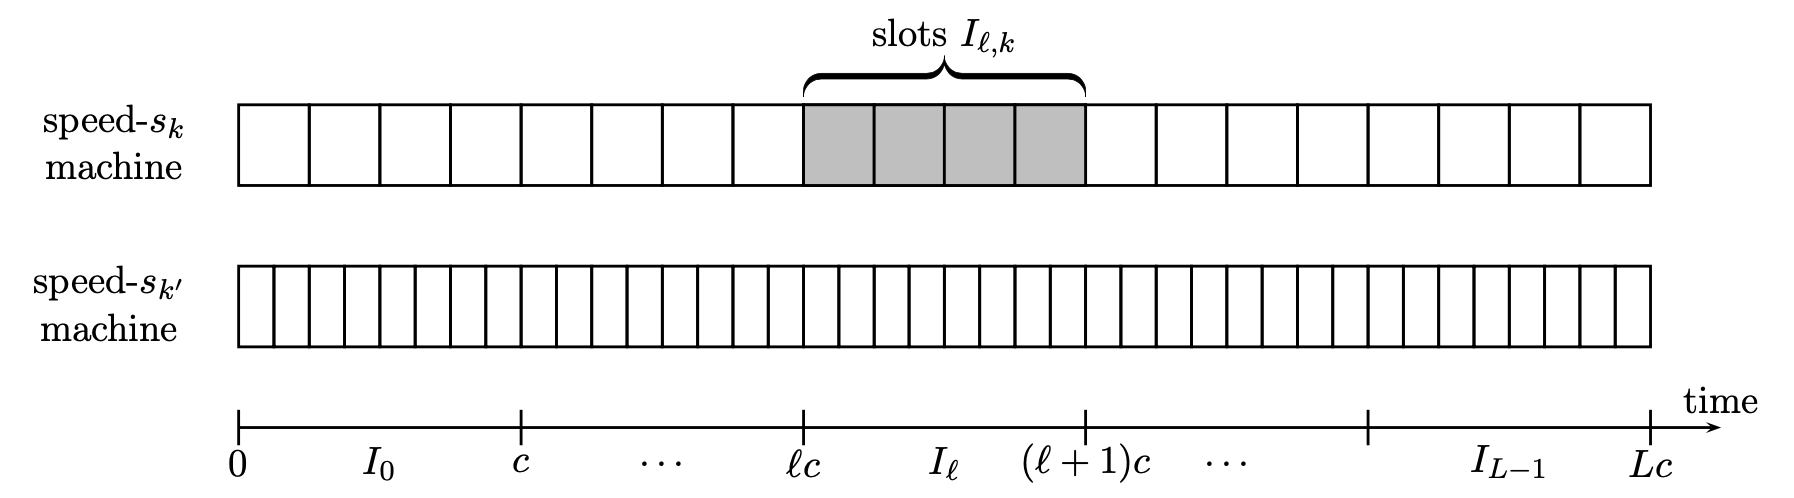
\includegraphics[width=15cm]{chapters/scheduling2/speed_slots}
%     \psset{xunit=0.7cm,yunit=0.8cm}
%     \begin{pspicture}(0,-0.5)(20,4.5)
%      \multido{\N=0+1}{20}{\rput[c](\N,3){\pspolygon(0,0)(1,0)(1,1)(0,1)}}
%      \multido{\N=8+1}{4}{\rput[c](\N,3){\pspolygon[fillcolor=lightgray,fillstyle=solid](0,0)(1,0)(1,1)(0,1)}}
%      \multido{\N=0.0+0.5}{40}{\rput[c](\N,1){\pspolygon(0,0)(0.5,0)(0.5,1)(0,1)}}
%      \psline{->}(0,0)(21,0) \rput[c](21,8pt){time}
%      \rput[r](-0.5,3.5){$\begin{array}{c} \textrm{speed-}s_k \\ \textrm{machine} \end{array}$}
%      \rput[r](-0.5,1.5){$\begin{array}{c} \textrm{speed-}s_{k'} \\ \textrm{machine} \end{array}$}
%      \psline(0,5pt)(0,-5pt) \rput[c](0,-10pt){$0$}
%      \psline(4,5pt)(4,-5pt) \rput[c](4,-10pt){$c$}
%      \psline(8,5pt)(8,-5pt) \rput[c](8,-10pt){$\ell c$}
%      \psline(12,5pt)(12,-5pt) \rput[c](12,-10pt){$(\ell+1)c$}
%      \psline(16,5pt)(16,-5pt) %\rput[c](12,-10pt){$(\ell+1)c$}
%      \psline(20,5pt)(20,-5pt) \rput[c](20,-10pt){$L c$}
%      \rput[c](2,-10pt){$I_0$}
%      \rput[c](6,-10pt){$\ldots$}
%      \rput[c](10,-10pt){$I_{\ell}$}
%      \rput[c](14,-10pt){$\ldots$}
%      \rput[c](18,-10pt){$I_{L-1}$}
     
%      \psbrace[rot=-90,ref=1C,nodesepB=-5pt,braceWidthInner=5pt,braceWidthOuter=5pt](12,4.1)(8,4.1){slots $I_{\ell,k}$}
%     \end{pspicture}
    \caption{Slots for different machine types.\label{fig:SlotsForMachineClasses}}
  \end{center}
  \end{figure}
  
  
  We construct the LP in two steps.
  First consider the variables
  \[
    x_{j,i,t} = \begin{cases} 1 & \textrm{if }j\textrm{ is scheduled on machine }i\textrm{ in time slot }t \in I_{*,k} \,, \\ 0 & \textrm{otherwise} \end{cases}
  \]
  for all $j \in J$, $k \in [M]$, $i \in [m_k]$, and $t \in I_{*,k}$.
  Let $K$ be the set of fractional solutions to the following linear system:
  \begin{eqnarray*}
    \sum_{k \in [M], i \in [m_k]} \sum_{t \in I_{*,k}} x_{j,i,t} &=& 1 \quad \forall j \in J \\
    \sum_{j \in J} x_{j,i,t} &\leq& 1 \quad \forall k \in [M] \;\; \forall i \in [m_k] \;\; \forall t \in I_{*,k} \\
    0 \leq x_{j,i,t} &\leq& 1 \quad \forall j \in J \; \forall k \in [M] \; \; \forall i \in [m_k] \; \forall t \in I_{*,k}
  \end{eqnarray*}
  
  
  We note that the assignment constraints are the set of equations 
  $\sum_{k \in [M], i \in [m_k]} \sum_{t \in I_{*,k}} x_{j,i,t} = 1$ for every $j \in J$.
  
  Next, we will use a lift $x \in \textsc{SA}_r(K)$, which contains in particular the variables
  $x_{(j_1,i_1,t_1),(j_2,i_2,t_2)}$ that provide the probability for the event that $j_1$ is scheduled at time $t_1$ on machine $i_1$ and
  $j_2$ is scheduled at time $t_2$ on machine $i_2$.
  We introduce more types of decision variables: 
  \begin{eqnarray*}
    y_{j_1,j_2,k} &=& \begin{cases} 1 & j_1\textrm{ and }j_2\textrm{ are scheduled on the same machine of type $k$ in the same interval,} \\ 0 & \textrm{otherwise,} \end{cases} \\
    y_{j_1,j_2} &=& \begin{cases} 1 & j_1\textrm{ and }j_2\textrm{ are scheduled on the same machine in the same interval,} \\ 0 & \textrm{otherwise,} \end{cases} \\
     C_j &=& \textrm{completion time of job }j.
  \end{eqnarray*}
  
  
  The LP relaxation is then as follows: 
  \begin{eqnarray*}
    \textrm{Minimize} & & \sum_{j \in J} w_j \cdot C_j  \quad \textsf{(LP)} \\
    y_{j_1,j_2,k} &=& \sum_{\ell \in \{ 0,\ldots,L-1\}}  \sum_{i \in [m_k]} \sum_{t_1 \in I_{\ell,k}} \sum_{t_2 \in I_{\ell,k}} x_{(j_1,i,t_1),(j_2,i,t_2)} \quad \forall j_1,j_2 \in J\; \forall k \in [M] \\
    y_{j_1,j_2} &=& \sum_{k}  y_{j_1,j_2,k}  \hspace{5.9cm} \forall j_1,j_2 \in J\\
    C_{j_2} &\geq& C_{j_1} + (1-y_{j_1,j_2}) \cdot c \hspace{4.3cm} \forall j_1 \prec j_2 \\
    C_j &=&  \sum_{k \in [M], i \in [m_k]} \sum_{t \in I_{*,k}} x_{j,i,t} \cdot t \hspace{3.7cm} \forall j \in J \\ 
    x &\in& SA_r(K)
  \end{eqnarray*}
  
  Following the discussion in Section~\ref{sec:SheraliAdamsHierarchy}, we know that for every job $j$, there is a
  distribution that we denote as $(\tilde{x},\tilde{y}) \sim \pazocal{D}(j^*)$ such that $\E[\tilde{x}_{j,i,t}] = x_{j,i,t}$
  and $\E[\tilde{y}_{j_1,j_2}] = y_{j_1,j_2}$ with $\tilde{x} \in SA_{r-1}(K)$ where job $j^*$ is integrally assigned and $(\tilde{x},\tilde{y})$ satisfies the first two constraints in $(\mathsf{LP})$.
  This is immediate for the $x$-part as $x \in SA_r(K)$, and follows for the $y$-variables as these  
  linear in the $x$-variables. 
  %In several proofs, we consider a solution drawn after conditioning on event. 
  %When we condition on a job $j$ being assigned integrally to a machine and time slot, we denote the corresponding solution and distribution as $(\tilde{x},\tilde{y}) \sim \pazocal{D}(j)$. 
  If $\pazocal{E}$ is an event, then we write $(\tilde{x},\tilde{y}) \sim \pazocal{D}(j^* \mid \pazocal{E})$ as the conditional distribution (conditioning on the event $\pazocal{E}$ occurring), see again Section~\ref{sec:SheraliAdamsHierarchy} for details.
  
  
  
  %#########LP Properties###################
  
  \subsection{Properties of the LP}
  \label{sec:LP-properties}
  
  We will now discuss some properties that are implied by the Sherali-Adams lift.
  The properties proved in this section, which we use crucially in our rounding algorithms, are the main technical contributions of this paper.
  
  \begin{lemma}\label{lem:Relmetric}
  Let $(x,y,C)$ be a solution to $(\mathsf{LP})$ with $r \geq 5$. Then $d(j_1,j_2) := 1-y_{j_1,j_2}$ is a semimetric.
  \end{lemma}
  This property was proven in \cite{DKRTZ20} for a special case of $s_k = 1$
  and is not hard to extend to our more general LP. From now on, the symbol $d$ as well as the quantity $\textrm{diam}( \cdot )$ will always refer to this particular semimetric. 
  For the special case of $s_k = 1$ for all $k$, one can also find a proof in \cite{DKRTZ20} that any set $U \subseteq J$ with $\textrm{diam}(U) \leq \frac{1}{2}$ has size $|U| \leq 2c$.
  While this is a obviously false for arbitrary speeds $s_k$, we can prove a similar claim: 
  %\begin{lemma}\label{lem:Rclustercapacity} % T: This lemma was not needed. 
  %For every $j_1 \in J$ and for every machine type $k \in [M]$, one has $\sum_{j_2 \in J} y_{j_1,j_2,k} \leq s_k \cdot c$.
  %\end{lemma}
  %The above lemmas are generalizations of the lemmas we proved for the identical machines case \cite{}, and we defer the proofs to appendix.
  \begin{lemma} \label{lem:BoundSumOfYj1j2kForFixedJ1}
  For $k \in [M]$ and $j_1 \in J$ one has $\sum_{j_2 \in J} y_{j_1,j_2,k} \leq s_k \cdot c \cdot \sum_{i \in [m_k]}\sum_{t}
  x_{j_1,i,t} \leq s_k \cdot c$.
  \end{lemma}
  \begin{proof}
    The second inequality is trivial as $\sum_{i \in [m_k]} \sum_{t} x_{j_1,i,t} \leq 1$, so we only justify the first inequality. 
  As we are proving a linear inequality, it suffices to show this for a fixed outcome $(\tilde{x},\tilde{y}) \sim \pazocal{D}(j_1)$ where job $j_1$ is assigned integrally. 
  If in $(\tilde{x},\tilde{y})$ the job $j_1$ is not assigned to a machine in $[m_k]$, then both sides are 0. 
  So suppose that $j_1$ is assigned to a machine $i_1 \in [m_k]$ and to interval $\ell_1$.
  Then indeed
  \[
  \sum_{j_2 \in J} \tilde{y}_{j_1,j_2,k} = \sum_{j_2 \in J} \sum_{t \in I_{\ell_1,k}} \tilde{x}_{j_2,i_1,t} \leq s_k c = s_k c \underbrace{\sum_{i \in [m_k]}\sum_{t} \tilde{x}_{j_1,i,t}}_{=1}
  \,.
  \]
  \end{proof}
  
  
  Lemmas~\ref{lem:RSmallNeighborhoodOfClosePoints} and \ref{lem:StrongerRSmallNeighborhoodOfClosePoints} are key technical insights  behind the algorithms for the related machines setting. They say that if one considers a set of jobs which are close to each other with respect to $d$,  then there exists a type $k^*$ such that we can schedule all the jobs in an interval of length $O(c)$ on a single machine of type $k^*$. Moreover, the LP also schedules a good fraction  of these jobs on the same machine type.
  These lemmas are important in assigning jobs to machine types in our algorithms.
  
  
  
  \begin{lemma}
  \label{lem:RSmallNeighborhoodOfClosePoints}
  Let $U \subseteq J$ be a non-empty subset of jobs with $\textrm{diam}(U) \leq \frac{1}{4}$. Then there exists a $k^* \in [M]$ such that
  \begin{enumerate*}
  \item[(i)] $|U| \leq O(1) \cdot s_{k^*} \cdot c$, and
  \item[(ii)] $\sum_{j \in U} \sum_{i \in [m_{k^*}]} \sum_t x_{j,i,t} \geq \Omega(\frac{1}{M}) \cdot |U|$.
  \end{enumerate*}
  \end{lemma}
  
  \begin{proof} 
  Let us sort the speed classes $[M]$ so that $s_1 \geq \ldots \geq s_M$ and abbreviate $z_{j,k} := \sum_{i \in [m_k]} \sum_t x_{j,i,t}$ as the fraction of job $j$ scheduled on class $k$.
  Moreover  let $\rho_{k} := \sum_{j \in U} z_{j,k}$ be the load of cluster $U$ on class $k$.
  We fix an arbitrary job $j^* \in U$. Let $k_{\textrm{median}} \in [M]$ be the median speed class for job $j^*$, meaning that $\sum_{k \leq k_{\textrm{median}}} z_{j^*,k} \geq \frac{1}{2}$ and $\sum_{k \geq k_{\textrm{median}}} z_{j^*,k} \geq \frac{1}{2}$. 
  We split the remaining proof into two separate claims. \\
  {\bf Claim I.} \emph{One has $|U| \leq  4 \cdot s_{k_{\textrm{median}}} \cdot c$.} \\
  {\bf Proof of Claim I.} First we observe that for every $j \in U$ we have $\sum_{k \geq k_{\textrm{median}}} y_{j^*,j,k} \geq \frac{1}{2}-d(j^*,j) \geq \frac{1}{4}$. 
  We use this to estimate
  \begin{eqnarray*}
  \frac{|U|}{4} &\leq&  \sum_{k \geq k_{\textrm{median}}}\sum_{j \in U} y_{j^*,j,k} \stackrel{\textrm{Lem~\ref{lem:BoundSumOfYj1j2kForFixedJ1}}}{\leq}
  \sum_{k \geq k_{\textrm{median}}} s_k c\sum_{i \in [m_k]}\sum_{t}
  x_{j^*,i,t} \\ &\leq& s_{k_{\textrm{median}}}c \underbrace{\sum_{k \geq
  k_{\textrm{median}}} \sum_{i \in [m_k]}\sum_t x_{j^*,i,t}}_{\leq 1} 
  \leq s_{k_{\textrm{median}}}c
  \end{eqnarray*}
  Rearranging gives $|U| \leq 4s_{k_{\textrm{median}}}c$ as claimed. \qed \\
  {\bf Claim II.} \emph{There is a class $k^* \in \{1,\ldots,k_{\textrm{median}}\}$ where $\rho_{k^*} \geq \frac{|U|}{4M}$.} \\
  {\bf Proof of Claim II.} For any job $j \in U$ we have $\sum_{k \leq k_{\textrm{median}}} z_{j,k} \geq (\sum_{k \leq k_{\textrm{median}}} z_{j^*,k}) - d(j,j^*) \geq \frac{1}{2} - \frac{1}{4} = \frac{1}{4}$.
  Hence $\sum_{k \leq k_{\textrm{median}}} \rho_k \geq \frac{|U|}{4}$.
  Then at least one index $k^* \in \{ 1,\ldots,k_{\textrm{median}}\}$ will have $\rho_{k^*} \geq \frac{|U|}{4M}$.
  \end{proof}
  
  %The above lemma guides in assigning clusters of jobs obtained via the CKR algorithm to machine types.
  While the above lemma is enough to obtain our approximation algorithm for  makespan on related machines, for the weighted completion time objective we need the following strengthening: if one considers a set of jobs which are {\em very} close to each other, then there exists a type $k^*$ such that we can schedule all the jobs in an interval of length $O(c)$ on a single machine of type $k^*$. 
  Moreover, the LP solution also schedules at least $\Omega(1/M)$ fraction of {\em every one of these jobs} on the same machine type.
  Recall that Lemma \ref{lem:RSmallNeighborhoodOfClosePoints} only satisfied this condition on average.
  
  % Recall that we use the notation $(\tilde{x},\tilde{y}) \sim \pazocal{D}(j^*)$ to obtain the distribution corresponding to the Sherali-Adams lift, where job $j^*$ is assigned integrally. 
  
  
  \begin{lemma}
  \label{lem:StrongerRSmallNeighborhoodOfClosePoints}
  Let $U \subseteq J$ be a non-empty set with $\textrm{diam}(U) \leq \frac{1}{8M}$ and abbreviate $z_{j,k} := \sum_{i \in [m_k]} \sum_{t} x_{j,i,t}$. Then
  \begin{enumerate*}
     \item[(i)] $|z_{j_1,k} - z_{j_2,k}| \leq \textrm{diam}(U) \leq
  \frac{1}{8M}$ for all $j_1,j_2 \in U$ and $k \in [M]$.
     \end{enumerate*}
     Moreover there are indices $\pi(U) \subseteq [M]$ such that
     \begin{enumerate}
     \item[(ii)] $z_{j,k} \geq \frac{1}{4M}$ for all $j \in U$ and $k \in \pi(U)$
     \item[(iii)] $\sum_{k \in \pi(U)} \min\{ z_{j,k} : j \in U\}
  \geq \frac{1}{2}$
     \item[(iv)] $|U| \leq 2 \cdot s_k \cdot c$ for all $k \in \pi(U)$.
     \end{enumerate}
  \end{lemma}
  
  
  \begin{proof}
  We prove the points in order.
  \begin{enumerate}
  \item[(i)] Actually we claim the stronger property of $|z_{j_1,k} - z_{j_2,k}| \leq d(j_1,j_2)$.
  Sample a distribution $(\tilde{x},\tilde{y}) \sim \pazocal{D}(j_1,j_2)$ and let $\sigma(j_1) \in [m]$ be the random variable that denotes the machine index with $\sum_t \tilde{x}_{j_1,\sigma(j_1),t}=1$ (similarly we define $\sigma(j_2)$). 
  Then we can see that
  \[
  |z_{j_1,k}-z_{j_2,k}| = |\Pr[\sigma(j_1) \in [m_k]] -
  \Pr[\sigma(j_2) \in [m_k]]| \leq |\Pr[\sigma(j_1) \neq \sigma(j_2)]|
  \leq d(j_1,j_2).
  \]
  \end{enumerate}
  Now we fix any job $j^* \in U$ and set $\pi(U) := \{ k \in [M] : z_{j^*,k} \geq \frac{1}{4M} \}$. 
  Then we continue the proof:
  \begin{enumerate}
  \item[(ii)] By (i) we know that for each $j \in U$ and $k \in \pi(U)$ we have $z_{j,k} \geq z_{j^*,k} - \frac{1}{8M} \geq \frac{1}{4M}$.
  \item[(iii)] We have
  
  \begin{eqnarray*}
  \sum_{k \in \pi(U)} \min\{ z_{j,k} : j \in U\} &\geq&
  \sum_{k \in \pi(U)} \Big(z_{j^*,k}-\frac{1}{8M}\Big) \\ &\geq&
  \underbrace{\sum_{k \in [M]} z_{j^*,k}}_{=1} - \sum_{k \in [M] \setminus
  \pi(U)} \underbrace{z_{j^*,k}}_{\leq 1/(4M)} - \frac{1}{8M}
  \underbrace{|\pi(U)|}_{\leq M} \geq \frac{1}{2}
  \end{eqnarray*}
  
  \item[(iv)] Fix a machine type $k \in \pi(U)$ and consider the event $\pazocal{E} := ``\sum_{i \in [m_k]}\sum_{t} \tilde{x}_{j^*,i,t}=1''$ (meaning the event that $j^*$ is assigned to a machine in class  $k$). 
  Note that $\Pr_{(\tilde{x},\tilde{y}) \sim \pazocal{D}(j^*)}[\pazocal{E}] = z_{j^*,k} \geq \frac{1}{4M}$. 
  %We study the conditional distribution  $(\tilde{x},\tilde{y}) \sim \pazocal{D}(j^* \mid \pazocal{E})$.
  Now, let $(\bar{x},\bar{y})$ be the Sherali-Adams lift (see Lemma~\ref{lem:SAconditioningOnGroupOfIndices}) conditioned on the event $\pazocal{E}$. Then trivially $\sum_{i \in [m_k]}\sum_t  \bar{x}_{j^*,i,t} = 1$. 
  As we have conditioned on an event with probability $z_{j^*,k} \geq \frac{1}{4M}$, the chance of other events cannot increase by more than a factor of $4M$ (see again Lemma~\ref{lem:SAconditioningOnGroupOfIndices}).
  In particular for $j \in U$ we have $1 - \bar{y}_{j^*,j} \leq 4M \cdot (1-y_{j^*,j}) = 4M \cdot d(j^*,j) \leq \frac{1}{2}$.
  As $\bar{y}_{j^*,j,k'} = 0$ for all $k' \neq k$ and $j \in U$ we can conclude that $\bar{y}_{j^*,j,k} \geq \frac{1}{2}$ for all $j \in U$.
  Finally by Lemma~\ref{lem:BoundSumOfYj1j2kForFixedJ1} we know that $\sum_{j \in J} \bar{y}_{j^*,j,k} \leq s_k c$ which then gives $|U| \leq 2s_kc$.
  \end{enumerate}
  \end{proof}
  
  As it is always the case when using the Sherali-Adams hierarchy in the context of approximation algorithms,
  it is a valid question how much of the power of the hierarchy is really needed. Some properties
  such as the triangle inequality from Lemma~\ref{lem:Relmetric} or the constraints from Lemma~\ref{lem:BoundSumOfYj1j2kForFixedJ1} could be enforced by simply adding them to the original LP. However at various places such as Lemmas~\ref{lem:StrongerRSmallNeighborhoodOfClosePoints}, \ref{lem:RAlphapointBound} and \ref{lem:RVolumeBound} our analysis makes heavily use of the local consistency provided by the hierarchy. It remains open whether there is a more efficient linear program, say only with the original
  variables $x_{i,j,t},y_{j_1,j_2},C_j$ that suffices.
  
  %#########Rounding Algorithm.###################
  \section{The Rounding Algorithm for $\Q \mid \Prec, p_j=1, c \mid \sum w_j C_j$}
  \label{sec:Rounding}
  
  
  In this section, we describe the rounding algorithm which proves our main technical result, Theorem~\ref{thm:LPcompletiontime}.
  We let $C_j^A$ denote the algorithm's completion time of job $j$.
  We denote $\Gamma^{-}(j)$ as the predecessors of $j$ and $\Gamma^+(j)$ as the successors, 
  and similarly $\Gamma^{-/+}(J') = \{ j \in J : \exists j' \in J' \textrm{ s.t. } j \in \Gamma^{-/+}(j') \}$. 
  
  \begin{theorem}
  \label{thm:LPcompletiontime}
  There is a polynomial-time randomized algorithm that,
  given a solution $(x,y,C)$ to (LP) for $r \geq 5$,
  produces a schedule with completion times 
  $\{C^A_j\}_{j \in J}$ such that $$\E[C^A_j] \leq O(M \cdot \log^2 n) \cdot C_j \leq O(\log ^3 n) \cdot C_j.$$
  \end{theorem}
  
  Before we describe our rounding algorithm, we set up some notation.
  Let $(x, y, C)$ be an optimal solution to the LP with $r \geq 5$.
  We partition the jobs based on their fractional completion times in the LP solution. 
  For any constant $a > 128$ set $\delta = \frac{1}{a \cdot M \cdot \log 2n }$. 
  Consider
  \begin{equation}
  J_0 := \left \{ j : C_j <  \delta  \cdot c \right \}
  \end{equation}
  
  and for $\gamma \geq 1$ define
  \begin{equation}
  \label{eq:jkdefinition}
  J_\gamma := \left \{ j : 2^{\gamma-1} \cdot \delta \cdot c \leq C_j <  2^{\gamma} \cdot \delta \cdot c \right \}
  \end{equation}
  
  
  \medskip
  Our rounding algorithm has the following steps:
  \begin{itemize}
  \item Schedule $J_0$ via the first batch scheduling algorithm given in Section \ref{sec:firstbatch}
  \item For $\gamma = 1, 2,\ldots$, schedule $J_\gamma$ via the intermediate scheduling algorithm  given in  Section \ref{sec:nextbatch}.
  \item Concatenate the schedules of $J_0, J_1, J_2, \ldots$.
  \end{itemize}
  
  
  We show that the expected completion time of every job in the above schedule satisfies Theorem \ref{thm:LPcompletiontime}. 
  We need the following scheduling subroutine for the rounding steps above.
  
  
  \begin{theorem} \label{thm:RelatedMakespan}
  Let $(x,y,C$) be a solution to the LP with $r \geq 5$ and let $T^* \in \mathbb{N}$.
  For some subset $J' \subset J$, suppose in the LP solution completion time $C_j \leq T^*$ for every job $j \in J'$.
  Then there is a randomized polynomial time algorithm that schedules all jobs such that $C^A_j \leq O(\log m \cdot \log n  \cdot T^*) + O(\log m \cdot c)$ for every job $j \in J'$.
   \end{theorem}
  
  Note that the above theorem immediately implies our result for the makespan minimization problem on related machines.
  We prove this theorem in Section \ref{sec:makespan}.
  
  
  \subsection{First Batch Scheduling}
  \label{sec:firstbatch}
  Here we give an algorithm for scheduling jobs in $J_0$.
  We define the \emph{$\alpha$-point} of job $j$ as the earliest time $t_j^*$ when 
  the LP solution has completed an $\alpha$-fraction of $j$. Formally,
  \begin{equation} \label{eq:RAlphaPoints}
    t^*_j := \min \left\{t' \in [T]:  \sum_{i=1}^{m}  \sum_{t \leq t'} x_{j,i,t} \geq \alpha \right\}.
  \end{equation}
  
  For $ \beta \leq 1/4M$, consider any subset $U \subseteq J$ with $\textrm{diam}(U) \leq \beta$.
  %$j^* \in J$, consider any $U := \{ j \in J \mid d(j,j^*) \leq \beta\}$.
  Let $\pi(U) \subseteq [M]$ denote the  indices of machine types that satisfy the conditions of Lemma \ref{lem:StrongerRSmallNeighborhoodOfClosePoints}.
  We use the same semimetric $d(j_1,j_2) := 1-y_{j_1,j_2}$ and schedule jobs in $J_0$ using the following algorithm.
  
  \begin{center}
   \fbox{
   \begin{minipage}{14cm}
    \textsc{First Batch Scheduling} \vspace{1mm} \hrule \vspace{1mm}
  \begin{enumerate*}
    \item[(1)] Run a CKR clustering on the semimetric space $(J_0,d)$ with parameter $\Delta := \frac{1}{100M}$ and let $V_1,\ldots,V_q$ be the clusters.
    \item[(2)] Let $V_{\ell}' := \{ j \in V_{\ell} \mid (\Gamma^-(j) \cap J_0) \subseteq V_{\ell}\}$ for $\ell = 1,\ldots,q$, and $J'_0 := \cup^{q}_{\ell = 1} V_{\ell}'$.
    \item[(3)] FOR $\ell = 1$ TO $q$ DO
          \begin{enumerate*}
            \item[(4)] Sample a machine type $k^*$ from the set $\pi(V'_\ell)$ with probability $\frac{\min \{z_{jk^*} : j \in V'_\ell \} }{\sum_{k \in \pi(V'_\ell)} \min \{z_{jk} : j \in V'_\ell \}}$.
            \item[(5)] Assign  $V'_\ell$ to a machine $i \in [m_{k^*}]$ with probability $\frac{1}{m_{k^*}}$.
           \end{enumerate*}
    \item [(6)] For a machine $i \in [m_k]$ of type $k$, let $J'_0(i,k)$ denote the set of jobs assigned to machine $i$.
    \item [(7)] For all $k$ and for all $i \in [m_k]$, schedule  $J'_0(i,k)$ in the increasing order of their $\alpha$-points for $\alpha = (1- \frac{1}{100M})$ as defined in Eq. (\ref{eq:RAlphaPoints}).
    \item[(8)] Insert a gap of $c$ time slots.
    \item[(9)] Let $J''_0 := J_0 \setminus J'_0$ be the set of jobs that did not get scheduled in steps (1) - (5). Use Theorem   \ref{thm:RelatedMakespan} to schedule $J''_0$.
    \end{enumerate*}
    \end{minipage}}
  \end{center}
  
  We now argue that expected completion time of a job $j$ in above algorithm is comparable to its LP cost.
  First we focus on bounding the completion time of jobs in $J'_0$.
  We need the following crucial lemma.
  
  \begin{lemma} 
  \label{lem:RAlphapointBound}
  %Let $\alpha = 1/100M$ be a small enough constant, and
  Let $U \subseteq J$ be a set of jobs  with $\textrm{diam}(U) \leq \frac{1}{100M}$ w.r.t. distance $d$. 
  For every job $j \in U$,  define $t_j^*$ as in Eq~\eqref{eq:RAlphaPoints}. 
  For $\theta > 0$, consider the set of jobs $U^* := \{ j \in U: t_j^* < \theta \} $ with $\alpha$-point less than $\theta$.  
  Then $|U^*| \leq 2 \cdot s_{k^*} \cdot \theta$ for any $k^* \in \pi(U)$.
   \end{lemma}
  
  The lemma formalizes the intuition that as the jobs in $U^*$ are very close to each other, it must be the case that the LP schedules all of them on the same machine.
  As a good fraction of each of these jobs are scheduled in the interval of length $\theta$ there cannot be too many of them.
  
  
  \begin{proof}
  We prove the lemma by contradiction.  Consider a set $U^*$ that violates the conditions in the lemma and fix a job $j^* \in U^*$.
  Let $k^* \in \pi(U)$.
  Then we have
    \begin{align*}
  (A) \;\; \sum_{j \in U^*} \sum_{i \in [m]} \sum_{t > \theta} x_{j,i,t}  < \frac{1}{100M} \cdot |U^*|, \quad &(B) \;\; \sum_{j \in U^*} y_{j,j^*} \geq \Big(1-\frac{1}{100M}\Big)|U^*|,\\ 
   \quad  &(C) \;\; \sum_{i \in [m_{k^*}]} \sum_{t \leq \theta} x_{j^*,i,t} \geq \frac{1}{5M}.
    \end{align*}
  where $(A)$ follows from the definition of $\alpha$-point of jobs, $(C)$ follows from  $\sum_{i \in [m_{k^*}]} \sum_{t=1}^{\theta} x_{j^*,i,t} \geq 1/4M - 1/100M > 1/5 M$, and
  $(B)$ follows from $\textrm{diam}(U^*) \leq \textrm{diam}(U) \leq \frac{1}{100M}$.
  Now we appeal to the properties of the Sherali-Adams hierarchy.
  Consider the event $\pazocal{E} := "\sum_{i \in [m_{k^*}]} \sum_{t \leq \theta} x_{j^*,i,t} = 1"$
  and note that from $(C)$ we know that the probability of the event $\pazocal{E}$ is at least $\frac{1}{5M}$.
  Now let $(\bar{x},\bar{y})$ be the Sherali-Adams lift with $\bar{x} \in SA_{r-1}(K)$ conditioned on this event, see Lemma~\ref{lem:SAconditioningOnGroupOfIndices} for details.
  In particular one has $\sum_{i \in [m_{k^*}]} \sum_{t \leq \theta} \bar{x}_{j^*,i,t} = 1$, meaning that the LP solution
  $(\bar{x},\bar{y})$ schedules $j^*$ fully on machines of class $k^*$ and until time $\theta$. 
  
  %We know that there is a distribution  $(\tilde{x},\tilde{y}) \sim \pazocal{D}(j^*)$ so that $\E[\tilde{x}_{j,i,t}] = x_{j,i,t}$ and $\E[\tilde{y}_{j_1,j_2}]=y_{j_1,j_2}$ while the variables involving job $j^*$ are integral, i.e. $\tilde{x}_{j^*,i,t} \in \{ 0,1\}$.
  %Now consider the conditional distribution  $(\tilde{x},\tilde{y}) \sim \pazocal{D}(j^* \mid \pazocal{E})$. 
  As we have conditioned on an event of probability at least $\frac{1}{5M}$, the probabilities of other events cannot increase by more than a factor of $5M$ (see the ``moreover'' part in Lemma~\ref{lem:SAconditioningOnGroupOfIndices}). 
  In particular for $j \in U$ we have $1 - \bar{y}_{j^*,j} \leq 5M \cdot (1-y_{j^*,j}) = 5M \cdot d(j^*,j) \leq \frac{1}{10}$.
  Similarly, $\sum_{j \in U^*} \sum_{i \in [m]} \sum_{t > \theta} \bar{x}_{j,i,t}  \leq 5M \cdot (\sum_{j \in U^*} \sum_{i \in [m]} \sum_{t > \theta} x_{j,i,t}) \leq 5M \cdot \frac{1}{100M} \cdot |U^*| \leq \frac{|U^*|}{10}$.
  Therefore we have 
    \[
  (A') \;\; \sum_{j \in U^*} \sum_{i \in [m_{k^*}]} \sum_{t > \theta} \bar{x}_{j,i,t}  \leq \frac{|U^*|}{10}, \quad (B')  \sum_{j \in U^*} \bar{y}_{j,j^*} \geq \frac{9}{10} \cdot |U^*|, \quad   (C') \sum_{i \in [m_{k^*}]} \sum_{t\leq \theta} \bar{x}_{j^*,i,t} = 1.
  \]
  Then by Markov's inequality there exists an outcome  $(\tilde{x},\tilde{y}) \sim \pazocal{D}_{\bar{y}}(j^*)$ where the job $j^*$ is integrally assigned and
    \[
  (A'') \;\; \sum_{j \in U^*} \sum_{i \in [m_{k^*}]} \sum_{t > \theta} \tilde{x}_{j,i,t}  \leq \frac{|U^*|}{5}, \quad (B'')  \sum_{j \in U^*} \tilde{y}_{j,j^*} \geq \frac{4}{5} \cdot |U^*|, \quad   (C'') \sum_{i \in [m_{k^*}]} \sum_{t \leq \theta} \tilde{x}_{j^*,i,t} = 1.
  \]
  We fix that outcome and let $i^* \in [m_{k^*}],t^* \in \{ 1,\ldots,\theta\}$ be the indices with $\tilde{x}_{j^*,i^*,t^*}=1$. Let $\ell^*$ be the interval index such that $t^* \in I_{\ell^*,k^*}$. 
  Then
  \begin{eqnarray*}
    \frac{4}{5} \cdot |U^*| &\stackrel{(B'')}{\leq}& \sum_{j \in U^*} \tilde{y}_{j,j^*} \stackrel{LP}{=} \sum_{j \in U^*} \sum_{\ell \in \{ 0,\ldots,L-1\}} \sum_{k} \sum_{i \in [m_k]} \sum_{t_1 \in I_{\ell,k}} \sum_{t_2 \in I_{\ell,k}} \tilde{x}_{(j,i,t_1),(j^*,i,t_2)} \\ 
    &\leq& \sum_{j \in U^*}\sum_{t \in I_{\ell^*,k^*}}\tilde{x}_{j,i^*,t}
    = \underbrace{\sum_{j \in U^*} \sum_{t \in I_{\ell^*,k^*}: t \leq \theta} \tilde{x}_{j,i^*,t}}_{\leq s_{k^*} \cdot \theta\textrm{ by LP}} + \underbrace{\sum_{j \in U^*} \sum_{t \in I_{\ell^*,k^*}:t > \theta^*} \tilde{x}_{j,i^*t}}_{\leq \frac{1}{5} \cdot |U^*| \textrm{ by }(A'')} \\
    &\leq& s_{k^*} \cdot \theta + \frac{|U^*|}{5}
  \end{eqnarray*}
  Rearranging gives $|U^*| \leq \frac{5}{3} \cdot s_{k^*} \cdot \theta^*$, which is a contradiction.
  \end{proof}
  
  
  \begin{lemma}
  \label{lem:RVolumeBound}
  Let $\theta > 0$ and $i$ be any machine of type $k$. Then with high probability $1-1/n^{100}$ it holds that
  $$
  | \{ j \in J'_0(i,k) : t^*_j \leq   \theta \} | \leq O\Big(\frac{\log n}{\log \log n} \cdot s_k \cdot \theta\Big)
  $$
   \end{lemma}
  \begin{proof}
  Fix $\theta^* > 0$ and any machine $i^*$ of type $k$. 
  Consider any outcome of the clustering itself. 
  The randomness needed for the lemma is only over the assignment in step (3)-(5) of the algorithm. We define the following random variables. Let
  \[
  X_{\ell}= \begin{cases}  | \{ j \in V'_{\ell} : t^*_j \leq   \theta^* \} | &\textrm{if } V'_{\ell} \textrm{ is assigned to machine} \hspace{1mm} i^* \hspace{1mm}   \textrm{of type} \hspace{1mm} k \hspace{1mm} \textrm{by our algorithm,} 
  \\ 0 & \textrm{otherwise} 
  \end{cases}
  \]
  and abbreviate $X = \sum^{q}_{\ell = 1} X_\ell$. Note the random variables $X_{1},\ldots,X_q$ are independent and $X = | \{ j \in J'_0(i^*,k) : t^*_j \leq   \theta^* \} |$.
  From Lemma \ref{lem:RAlphapointBound} we know that $X_\ell \leq 2s_k \cdot \theta^*$ for all $\ell$.
  
  Next, we estimate $\E[X]$. Recall that the algorithm uses the indices $\pi(V_{\ell}') \subseteq [M]$ from Lemma~\ref{lem:StrongerRSmallNeighborhoodOfClosePoints} 
  which in particular satisfy $z_{j,k} \geq \frac{1}{4M}$ and $|z_{j,k}-z_{j',k}| \leq \frac{1}{8M}$ whenever $j,j' \in V_{\ell}'$ with $k \in \pi(V_{\ell}')$.
  Abbreviate
  \[
    \mu_{\ell,k} := \begin{cases} \min\{ z_{j,k} : j \in V_{\ell}' \} & \textrm{if }k \in \pi(V_{\ell}') \\
      0 & \textrm{otherwise.} \end{cases}
  \]
  Recall that for every $\ell$ we have $\sum_{k \in [M]} \mu_{\ell,k} \geq 1/2$. We prove two technical claims that we need for our analysis: \\
  {\bf Claim I.} \emph{For any $\ell$ and $k$ and $j \in V_{\ell}'$ one has $\mu_{\ell,k} \leq 2z_{j,k}$.} \\
  {\bf Proof of Claim.} If $k \notin \pi(V_{\ell}')$ then the left hand side is 0, so suppose  $k \in \pi(V_{\ell}')$. Then $\mu_{\ell,k} = \min\{ z_{j',k} : j' \in V_{\ell}'\} \leq z_{j,k} + \frac{1}{8M} \leq 2z_{j,k}$. \qed \\
  {\bf Claim II.} \emph{For $j \in V_{\ell}'$ with $t_j^* \leq \theta^*$ and $k \in \pi(V_{\ell}')$ one has $z_{j,k} \leq 2 \sum_{i \in [m_k]} \sum_{t \in I_{*,k}: t \leq \theta^*} x_{j,i,t}$.}
  {\bf Proof of Claim II.} Since $k \in \pi(V_{\ell}')$ we know that $z_{j,k} \geq \frac{1}{4M}$.
  We consider the distribution $(\tilde{x},\tilde{y}) \sim \pazocal{D}(j)$ and denote $\tilde{i}$ and $\tilde{t}$ as the random indices so that $\tilde{x}_{j,\tilde{i},\tilde{t}}=1$. Then $\Pr[\tilde{i} \in [m_k]] = z_{j,k}$ and $\Pr[\tilde{t} > \theta^*] = \sum_{k \in [M]} \sum_{i \in [m_k]} \sum_{t \in I_{*,k}: t > \theta^*} x_{j,i,t} \leq \frac{1}{100M}$ by the definition of $\alpha$-points and the assumption $t_{j}^* \leq \theta^*$. Then
  \begin{eqnarray*}
    \sum_{i \in [m_k]} \sum_{t \in I_{*,k}: t \leq \theta^*} x_{j,i,t} &=& \Pr\big[\tilde{i} \in [m_k]\textrm{ and }\tilde{t} \leq \theta^*\big] \\
    &\geq&  \Pr\big[\tilde{i} \in [m_k]\big] - \Pr\big[\tilde{t} > \theta^*\big] \\
    &\geq& z_{j,k} - \frac{1}{100M} \geq \frac{1}{2}z_{j,k} \quad \quad \qed
  \end{eqnarray*}
  
  Now we can bound the expectation of our random variable as
  \begin{eqnarray*}
    \E[X] &=& \frac{1}{m_k} \sum_{\ell=1}^q \Pr\big[V_{\ell}'\textrm{ assigned to class }k\big] \cdot |\{j \in V_{\ell}': t_j^* \leq \theta^*\}| \\
          &=& \frac{1}{m_k} \sum_{\ell=1}^q \frac{\mu_{\ell,k}}{\sum_{k'} \mu_{\ell,k'}} \cdot |\{j \in V_{\ell}': t_j^* \leq \theta^*\}| \\
    &\stackrel{\textrm{Claim I}}{\leq}& \frac{4}{m_k} \sum_{\ell: k \in \pi(V_{\ell}')} \sum_{j \in V_{\ell}': t_j^* \leq \theta^*} z_{j,k} \\
          &\stackrel{\textrm{Claim II}}{\leq}& \frac{8}{m_k} \sum_{\ell: k \in \pi(V_{\ell}')} \sum_{j \in V_{\ell}': t_j^* \leq \theta^*} \sum_{i \in [m_k]} \sum_{t \in I_{*,k}: t \leq \theta^*} x_{j,i,t} \\
   &\leq& \frac{8}{m_k} \sum_{i \in [m_k]} \sum_{t \in I_{*,k}: t \leq \theta^*} \underbrace{\sum_{j \in J_0'}  x_{j,i,t}}_{\leq 1\textrm{ by }(\mathsf{LP})} \leq 8 \cdot |\{ t \in I_{*,k}: t \leq \theta^*\}| \leq 8s_k \cdot \theta^*
  \end{eqnarray*}
  Here we also have used that $\sum_{k' \in [M]} \mu_{\ell,k'} \geq \frac{1}{2}$. 
  As $X$ is sum of independent random variables $X_\ell$ each of which is bounded by $O(s_k \cdot \theta^*)$, we apply the Chernoff bound from Lemma~\ref{lem:ChernoffBound} and obtain that $\Pr[X > C' \cdot \frac{\log n}{\log \log n} \cdot s_k \theta^*] \leq 1/n^{1000}$ for some constant $C'>0$.
  To complete the lemma, we simply do a union bound over all possible values of $\theta^*$ and $i$. The number of machines is $m \leq n$ and the number of relevant $\theta^*$'s in the time horizon is bounded by $\sum_{k \in [M]} |I_{*,k}| \leq M \cdot 2n$.
  \end{proof}
  % \begin{proof}
  % Fix $\theta^* \in \mathbb{N}$ and any machine $i^*$ of type $k$. \rem{T: Actually $\theta$ would be over all relevant times, but they do not need to be integer. }
  % Consider any outcome of the clustering itself. 
  % The randomness needed for the lemma is only over the assignment in step (3)-(5) of the algorithm. We define the following random variables. Let
  % \[
  % X_{\ell}= \begin{cases}  | \{ j \in V'_{\ell} : t^*_j \leq   \theta^* \} | &\textrm{if } V'_{\ell} \textrm{ is assigned to machine} \hspace{1mm} i^* \hspace{1mm}   \textrm{of type} \hspace{1mm} k \hspace{1mm} \textrm{by our algorithm,} 
  % \\ 0 & \textrm{otherwise} 
  % \end{cases}
  % \]
  % and abbreviate $X = \sum^{q}_{\ell = 1} X_\ell$. Note the random variables $X_{1},\ldots,X_q$ are independent and $X = | \{ j \in J'_0(i^*,k) : t^*_j \leq   \theta^* \} |$.
  % From Lemma \ref{lem:RAlphapointBound} we know that $X_\ell \leq 2s_k \cdot \theta^*$ for all $\ell$.
  
  % Let $ V^*$ be the set of all clusters that are assigned to machines of type $k$ by our algorithm,
  % and define $J_{\theta^*}(k) := \{j \in V^*:  t^*_j \leq \theta^* \}$.  
  % From the capacity constraints of the LP we know that $\sum_{j \in J_\theta^*(k)} z_{jk} \leq m_k \cdot s_k \cdot \theta^*$. \rem{T: This is not right mathematically. Due to the change in the algorithm, $V^*$ is a random set and $J_{\theta^*}(k)$. Then  $\sum_{j \in J_\theta^*(k)} z_{jk} \leq m_k \cdot s_k \cdot \theta^*$ isn't true (it might hold in expectation)}
  
  % Our algorithm assigns a cluster $V'_{\ell}$ to the machine $i^*$ if it satisfies the conditions of  Lemma \ref{lem:StrongerRSmallNeighborhoodOfClosePoints}. 
  % Then, $V'_{\ell}$ is assigned to $i^*$ with probability
  % $$
  % \frac{1}{m_k} \cdot \frac{\min \{z_{jk} : j \in V'_\ell \} }{\sum_{j \in V'_\ell} \min \{ z_{jk} : j \in V'_\ell \}} \leq \frac{1}{m_k}  \cdot 2  \cdot \min \{z_{jk} : j \in V'_\ell \}
  % $$
  % This further implies that a job $j \in J_\theta^*(k)$ is assigned to the machine $i^*$ with probability at most $z_{jk}/m_k$.
  % Now we can bound the expectation of random variable $X$. Consider,
  % $$
  % \E[X] =  \sum_{j \in J_\theta^*(k)} \textrm{Pr [$j$ is assigned to $i^*$]} \leq  \frac{2}{m_k} \cdot \sum_{j \in J_\theta^*(k)} z_{jk} = \frac{2}{m_k} \cdot  (m_k \cdot s_k \cdot \theta^*) \leq 2s_k \cdot \theta^* 
  % $$
  % As $X$ is sum of independent random variables $X_\ell$ each of which is bounded by $O(s_k \cdot c)$ by  Lemma \ref{lem:RAlphapointBound}, we apply the Chernoff bound from Lemma~\ref{lem:ChernoffBound} to argue that $\Pr[X > C' \cdot \frac{\log n}{\log \log n} \cdot s_k c] \leq 1/n^{1000}$ for some constant $C'>0$.
  % To complete the lemma, we simply do a union bound over all possible values of $\theta$ and $i$, both of which are bounded by $O(n)$. \rem{T: This has to be for all possibly relevant times and the upperbound that I see is $\sum_k |I_{0,k}| \leq c\sum_k s_k$. This isn't quite linear in $n$.}
  % \end{proof}
  
  
  \begin{lemma}
  \label{lem:completiontimeJ'_0}
  For every job $j \in J'_0$, with high probability, the completion time of $j$ in our schedule $C^{A}_j \leq O( M \cdot \frac{\log n}{\log \log n} \cdot C_j)$.
  \end{lemma}
  \begin{proof}
  Fix a job $j^* \in J'_0$, and suppose job $j^*$ is scheduled on machine $i$ of type $k$ in our schedule.
  From Lemma \ref{lem:RVolumeBound}, there are at most $O( \frac{\log n}{\log \log n} \cdot s_k \cdot t^*_{j^*})$ jobs whose $t^*_j \leq t^*_{j^*}$.
  Therefore, the completion time is  $C^A_{j^*} \leq O(\frac{\log n}{\log \log n} \cdot t^*_{j^*})$.
  Note that in the LP solution at least an $\frac{1}{100M}$-fraction of $j^*$ was scheduled at or after $t^*_{j^*}$.
  Hence, $C_j \geq \frac{1}{100M} \cdot t^*_{j^*}$.
  Putting things together we conclude  $C^{A}_j \leq O(\frac{\log n}{\log \log n} \cdot t_{j^*}^*) \leq O( M \cdot \frac{\log n}{\log \log n} \cdot C_j)$.
  \end{proof}
  
  
  
  Now we focus on bounding the completion time of jobs in $J''_0$. 
  
  \begin{lemma}
  \label{lem:completiontimeJ''_0}
  For every job $j \in J''_0$, the completion time of $j$ in our schedule $C^{A}_j \leq O( \log n \cdot c)$.
  \end{lemma}
  \begin{proof}
  From the definition of set $J_0$, for all $j \in J''_0$ the completion time $C_j \leq c \cdot \delta$ in the LP solution.
  This implies that at least a 1/2-fraction of every job $j \in J''_0$ is scheduled in the interval $[0, 2c \cdot \delta]$ in the LP solution.
  We take the LP solution restricted to $J''_0$ in the interval $[0, c \cdot \delta]$, and  invoke Theorem \ref{thm:RelatedMakespan} to construct a schedule of jobs $J''_0$.
  Theorem \ref{thm:RelatedMakespan} guarantees that every job  $j \in J''_0$ is scheduled in an interval of length at most $2c \cdot \delta \cdot (\log m \cdot \log n + M^2) + O(\log m \cdot c) = O(\log m \cdot c)$ from our choice of $\delta$.
  To complete the proof, it remains to account for the increase in completion time caused by jobs in  $J'_0$ as 
  our algorithm schedules $J''_0$ after scheduling jobs in $J'_0$.
  However, from Lemma \ref{lem:completiontimeJ'_0} every job in $J'_0$ has completion time at most $O(\log n \cdot c)$.
  Thus the lemma follows.
  \end{proof}
  
  \begin{lemma}\label{l:notin}
  For any job $j_1 \in J_0$, the probability that $j_1 \in J''_0$  is at most  $O(M \cdot \log n  \cdot \frac{C_{j_1}}{c})$.
  \end{lemma}
  \begin{proof}
    Consider the set $U := \{ j_1 \} \cup (\Gamma^{-}(j_1) \cap J_0)$ of $j_1$ and its ancestors. If $j_0 \prec j_1$, then $0 \leq C_{j_0} + c \cdot d(j_0,j_1) \leq C_{j_1}$ by the LP constraints and so $d(j_0,j_1) \leq \frac{C_{j_1}}{c}$.
    Then the diameter of $U$ with respect to semimetric $d$ is bounded by $2C_{j_1}/c$ and hence by Theorem~\ref{thm:ProbUSeperatedByClustering}.(b) the probability that $U$ is separated is bounded by $\ln(2n) \cdot \frac{4 \textrm{diam}(U)}{\Delta} \leq O(M \cdot \log n  \cdot \frac{C_{j_1}}{c})$.
  \end{proof}
  
  We can now bound the expected completion time of every job in $J_0$.
  \begin{lemma}
  \label{lem:completiontimeJ0}
  For every job $j \in J_0, \E[C^A_j] \leq O(M \cdot \log^2 n ) \cdot C_j$.
  \end{lemma}
  \begin{proof} 
  Fix a job $j_1 \in J_0$ and consider
  \begin{eqnarray*}
  \E[C^A_{j_1}]  &=& \E[C^A_{j_1} | (j_1 \in J'_0)] \cdot \text{Pr}[ (j_1  \in J'_0)] + \E[C^A_{j_1} | (j_1  \in J''_0)] \cdot \text{Pr}[ (j_1 \in J''_0)]  \\
  &\stackrel{(*)}{\leq}& O\Big( M \cdot \frac{\log n}{\log \log n} \cdot C_{j_1}\Big) +  O\Big(M \cdot \log n \cdot \frac{C_{j_1}}{c}\Big) \cdot O( \log n \cdot c)   \\
  &\leq& O(M \cdot \log^2 n) \cdot C_{j_1}, 
  \end{eqnarray*}
  where (*) follows from Lemmas  \ref{lem:completiontimeJ'_0}, \ref{lem:completiontimeJ''_0}, \ref{l:notin}.
  \end{proof}
  We also note the following simple consequence of previous lemmas:
  
  \begin{lemma}
  \label{lem:makespanofJ0}
  For every job $j \in J_0$, $C_j \leq O(\log n \cdot c)$.  In other words,  the makespan of our schedule for $J_0$ is at most $O(\log n \cdot c)$.
  \end{lemma}
  
  
  \subsection{Intermediate Batch Scheduling}
  \label{sec:nextbatch}
  Now we describe our algorithm to schedule jobs in the set $J_\gamma$ for $\gamma > 0$, which is  similar to that of scheduling jobs in $J''_0$.
  Recall that from the definition of set $J_\gamma$ in Eq. (\ref{eq:jkdefinition}), $2^{\gamma-1} \delta \cdot c  < C_j \leq  2^\gamma \delta \cdot c$ in the LP solution.
  We take the LP solution restricted to $J_\gamma$ in the interval $[0, 2^\gamma \delta \cdot c]$, and  invoke Theorem \ref{thm:RelatedMakespan} to construct a schedule of jobs $J_\gamma$.
  Theorem \ref{thm:RelatedMakespan} ensures that every job  $j \in J_\gamma$  is scheduled in an interval of length at most $O(2^\gamma \delta \cdot c \cdot \log m \cdot \log n) + O(\log n \cdot c)$. 
  As a consequence, we obtain the following lemma.
  \begin{lemma}
  \label{lem:intermediate}
  Fix any $\gamma^* \geq 0$. For every $j \in J_{\gamma^*}$, $C^A_j \leq O(2^{\gamma^*} \cdot \delta \cdot \log m \cdot \log n) + O(\gamma^* \cdot \log n \cdot c)$.
  \end{lemma}
  \begin{proof} 
  For $\gamma = 0, 1, \ldots$, let $\pazocal{S}(J_\gamma)$ denote the schedule of jobs in the set $J_\gamma$.
  Our final schedule $\pazocal{S}$ is simply a concatenation of schedules $\pazocal{S}(J_0), \pazocal{S}(J_1), \ldots$, while inserting $c$ empty time slots between  $\pazocal{S}(J_\gamma)$ and $ \pazocal{S}(J_{\gamma+1})$.
  Let $T_{\gamma}$ denote the makespan of $\pazocal{S}(J_\gamma)$.
  From Lemma \ref{lem:makespanofJ0} and Theorem \ref{thm:RelatedMakespan}, $T_{\gamma} \leq O(2^\gamma \cdot  \delta \cdot c \cdot \log m \cdot \log n ) + O(\log n \cdot c)$.
  Fix the job $j^* \in J_{\gamma^*}$ with the highest completion time in $\pazocal{S}$.
  We can bound the completion time of $j^*$ as
  
  \begin{eqnarray*}
  C^A_{j^*} &\leq& \sum^{\gamma^*}_{\gamma = 0} T_{\gamma} \leq  O(\gamma^* \cdot \log n \cdot c) + \sum^{\gamma^*}_{\gamma = 1} O(2^\gamma \cdot \delta \cdot c \cdot \log m \cdot \log n) \\
  &\leq& O(\gamma^* \cdot \log n \cdot c) + O(2^{\gamma^*} \cdot \delta \cdot c \cdot \log m \cdot \log n)
  \end{eqnarray*}
  which completes the proof.
  \end{proof}
  
  We finish the proof of main theorem for the weighted sum of completion times of jobs.
  
  \begin{proof} [Proof of Theorem \ref{thm:LPcompletiontime}]
  For every job $j \in J_0$, from Lemma \ref{lem:completiontimeJ0},  we have $\E[C^A_j] \leq O(M \cdot \log^2 n) \cdot C_j$.
  From the previous Lemma \ref{lem:intermediate}, for $\gamma  > 0$ and $j \in J_{\gamma }$ we have, $C^A_j \leq O(\gamma \cdot \log n \cdot c) + O(2^{\gamma } \cdot \delta \cdot c \cdot \log m \cdot \log n )$.
  On the other hand,  for every $j \in J_{\gamma}$, by definition, $C_j >  2^{\gamma} \cdot \delta \cdot c$.
  Thus, $C^A_j \leq  O(M \cdot \log^2 n) \cdot C_j$.
  \end{proof}
  
  
  %****************
  
  \section{Proof of Theorem \ref{thm:RelatedMakespan}}
  \label{sec:makespan}
  
  Recall that we are given a subset of jobs $J' \subseteq J$, and a solution $(x,y,C)$ to the LP with $r \geq 5$ and  $T \in \mathbb{N}$.
  It is promised that in  $(x,y,C)$, the completion times satisfy $C_j \leq T$ for every job $j \in J'$.
  Then there is a randomized polynomial time algorithm that schedules all jobs such that $C_j^A \leq O(\log m  \cdot \log n  \cdot T) + O(\log m \cdot c)$ for every job $j \in J'$. 
  %\rem{T: I added $C_j^A$ for the completion time of our algo.}
  
  \subsection{Main Scheduling Subroutine}
  \label{subsec:singlebatchrelated}
  
  The following lemma is the main scheduling subroutine towards proving Theorem \ref{thm:RelatedMakespan}. 
  
  \begin{lemma} \label{lem:RSchedulingOneIntervalViaCKR}
  Let $C^* \geq 0$ and $\delta = 1/64\log(2n)$. 
  Consider the set $J^* \subseteq \{ j \in J' \mid C^* \leq C_j \leq C^*+\delta \cdot c \}$.
  Then there is a randomized rounding procedure that finds a subset $J^{**} \subseteq J^*$,
  a partition of $J^{**}$ into $J^{**} = \cup_{k=1}^{M} J^{**(k)}$ where $J^{**(k)}$ are jobs assigned to machines of type $k$,
  and a schedule for $J^{**}$ in an interval of length at most $5c+\sum_k \frac{|J^{**(k)}|}{s_k \cdot m_k}$ such that every job $j \in J^*$
  is scheduled with probability at least $\frac{1}{2}$.
  \end{lemma}
  
  
  The rounding algorithm to prove the above lemma is the following:
  
  \begin{center}
  \fbox{
  \begin{minipage}{14cm}
    \textsc{Scheduling a Single Batch on Related Machines} \vspace{1mm} \hrule \vspace{1mm}
  \begin{enumerate*}
    \item[(1)] Run a CKR clustering on the semimetric space $(J^*,d)$ with parameter $\Delta := \frac{1}{4}$ and let $V_1,\ldots,V_q$ be the clusters.
    \item[(2)] Let $V_{\ell}' := \{ j \in V_{\ell} \mid \Gamma^-(j) \cap J^* \subseteq V_{\ell}\}$ for $\ell = 1,\ldots,q$.
    \item[(3)] For all $\ell=1,\ldots,q$, assign the jobs in $V_{\ell}'$ to type $k^*$ satisfying the conditions in Lemma \ref{lem:RSmallNeighborhoodOfClosePoints}.
    \item[(4)] For all $\ell=1,\ldots,q$, if $V_{\ell}'$ is assigned to type $k^*$, assign all jobs in $V_{\ell}'$ to the machine of type $k^*$ which has the least load (breaking ties arbitrarily). 
    \end{enumerate*}
     \end{minipage}}
  \end{center}
  
  We prove few lemmas that will be helpful in proving the desired properties of the algorithm.
  The first lemma shows that the clusters produced by the algorithm are not too large.
  
  \begin{lemma}
      \label{lem:RClusterSize}
  For all $\ell=1,\ldots,q$, one has $|V_{\ell}'| \leq O(s_{k^*}c)$. Here, $k^*$ is the machine type that $V_{\ell}'$ is assigned in our algorithm. Thus, it takes $O(c)$ time to process all jobs in $V_{\ell}'$. 
  \end{lemma}
  \begin{proof}
    We know by Theorem~\ref{thm:ProbUSeperatedByClustering} that $\textrm{diam}(V_{\ell}') \leq \textrm{diam}(V_{\ell}) \leq \Delta \le \frac{1}{4}$.
    The lemma follows by Lemma~\ref{lem:RSmallNeighborhoodOfClosePoints} and by our choice of $k^*$. 
  \end{proof}
  
  Further it is easy to see that the clusters respect precedence constraints.
  \begin{lemma}
  \label{lem:ClusterIndependence}
  The solution $V_{1}',\ldots,V_{q}'$ is feasible in the sense that jobs on different machines do not have precedence constraints.
  \end{lemma}
  \begin{proof}
    Consider jobs processed on different machines, say (after reindexing) $j_1 \in V_{1}'$ and $j_2 \in V_2'$.
     If $j_1 \prec j_2$ then we did \emph{not} have $\Gamma^-(j_2) \subseteq V_2'$. This contradicts
    the definition of the sets $V_{\ell}'$.
  \end{proof}
  
  
  We will use the two statements above together with Theorem~\ref{thm:ProbUSeperatedByClustering} to prove Lemma~\ref{lem:RSchedulingOneIntervalViaCKR}.
  
  \begin{proof}[Proof of Lemma~\ref{lem:RSchedulingOneIntervalViaCKR}]
  
    Call the schedule produced by the above algorithm $\pazocal{S}(J^*)$.
    By Lemma~\ref{lem:RClusterSize}, for all $\ell=1,\ldots,q$, the processing time of $V_{\ell}' $ is at most $O(c)$.
    By Lemma~\ref{lem:ClusterIndependence}, there are no dependent
    jobs in different sets of $V_1',\ldots,V_q'$. 
  
    
    The interval in which the jobs in $J^*$ are scheduled can be divided into $c$-length time intervals $I_1,\cdots,I_{\ell}$. 
    To prove the lemma, it suffices to consider the case where $\ell \ge 6$.
    We say that a machine of type $k$ is \emph{full} in a $c$-length interval if it is processing $c \cdot s_k$ jobs in $\pazocal{S}(J^*)$.
    From our greedy packing and the bound on processing time of $V_{\ell}'$, it follows that there exists a machine type $k \in [M]$ such that every machine $i \in [m_k]$ is full in $I_1, \cdots I_{\ell-5}$.
    Therefore, 
    \[c\cdot(\ell -5) \le \max_{k}\frac{|J^{**(k)}|}{s_k \cdot m_k} \le\sum_{k}\frac{|J^{**(k)}|}{s_k \cdot m_k}.
    \]
    
    Thus, the total length of the interval used in a single batch scheduling is bounded by
    \[ c\cdot \ell \le 5c+ \sum_{k}\frac{|J^{**(k)}|}{s_k \cdot m_k}.
    \]
  
  
  It remains to prove that a fixed job $j^* \in J^*$ is scheduled with good probability.
  Consider the set $U := \{ j^* \} \cup (\Gamma^-(j^*) \cap J^*)$ of $j^*$ and its ancestors in $J^*$.
  By the LP constraint $C_{j_1} + d(j_1,j_2) \cdot c \leq C_{j_2}$, rearranging we see that $d(j_1,j_2)  \leq \delta$ for every $j_1, j_2 \in U$.   
  So the diameter of $U$ is at most $2\delta$.
  Now we appeal to Lemma~\ref{lem:RSmallNeighborhoodOfClosePoints}.
  %to see that $ |N(U, \Delta/2)| \leq \frac{c}{1- 2\delta-  \Delta}$.
  For our choice of $\Delta = 1/4$ and $\delta \leq \frac{1}{64 \log(2n) }$,
  we apply Theorem~\ref{thm:ProbUSeperatedByClustering} to see that
  the cluster is separated with probability at most 
   $\log(2n) \cdot  \frac{8 \delta}{\Delta} \leq \frac{1}{2}$.
  \end{proof}
  
  To schedule all jobs in $J^*$, we repeat the clustering procedure $O(\log m)$ times and simply schedule the remaining jobs on the fastest machine. 
  
  \begin{lemma} \label{lem: FullSchedulingOneIntervalViaCKRForRelated}
    Let $C^* \geq 0$ and $\delta = 1/64\log(2n)$. 
  Consider the set $J^* \subseteq \{ j \in J' \mid C^* \leq C_j \leq C^*+\delta \cdot c\}$.
    Then there is an algorithm with expected polynomial running time that finds disjoint subsets  $J^{*(k)} \subset J^*$, 
    where $J^{*(k)}$ are jobs assigned to machines of type $k$, 
    and schedules all jobs in $J^*$ using at most $O(\log m \cdot c ) + \frac{|J^*|}{m\cdot s_{\max}}+\sum_k \frac{|J^{*(k)}|}{s_k \cdot m_k}$ many time slots.
  \end{lemma}
  
  \begin{proof}
  We run the above algorithm for $2 \log m$ iterations. Input to iteration $h+1$ is the set of jobs that are not scheduled in the first $h$ iterations. 
  For $h \in \{1,2,\ldots, 2 \log m \}$, let $J^{**}_{h}$ be the set of jobs scheduled in iteration $h$, and let $J^*_{h+1} := J^* \setminus \{ \bigcup^{h}_{i = 1} J^{**}_i$\}.
   In this notation,  $J^*_1 := J^*$.
  
   Let $\pazocal{S}(J^{**}_{h})$ be the schedule of jobs $J^{**}_{h}$ obtained from by Lemma~\ref{lem:RSchedulingOneIntervalViaCKR}.
    We schedule $\pazocal{S}(J^{**}_1)$ first, then append schedule $\pazocal{S}(J^{**}_{h})$ after $\pazocal{S}(J^{**}_{h-1})$ while inserting $c$ empty time slots between them, for $h = 2,\ldots, 2 \log m$.
   Let $\hat{J} := J^{*}_{2\log m +1}$ be the set of jobs that were not scheduled in these $2\log m$ iterations.
   We schedule all jobs in $\hat{J}$ consecutively on a single machine with the {\em fastest speed} after the completion of $\pazocal{S}(J^{**}_{2 \log m})$.
   
   From our construction, the length of a schedule for  $J^*$, which is a random variable, is at most $O(\log m \cdot c) +  \lceil \frac{|\hat{J}|}{s_{\max}} +\sum_k \frac{|J^{*(k)}|}{s_k \cdot m_k} \rceil$.
   For $h \in \{ 1,2, \ldots ,2\log m\}$,  Lemma~\ref{lem:RSchedulingOneIntervalViaCKR}  guarantees that each job $j \in J^*_{h}$ gets scheduled in the $h^{th}$ iteration with probability at least $1/2$.
   Therefore, the probability that $j \in \hat{J}$,  i.e. it does not get scheduled in the first $2 \log m$ iterations, is at most $\frac{1}{2m}$.
   This implies that $\mathbb{E}[|\hat{J}|] \leq \frac{|J^*|} {2m}$.
   The claimed expected polynomial running time bound now simply follows from appealing to Markov's inequality. 
  
   
   Finally, by our construction precedence and communication delay constraints are satisfied.
  \end{proof}
  
  \subsection{The Complete Algorithm}
  
  To schedule all jobs in $J'$ we do the following.
  \begin{center}
      \fbox{
          \begin{minipage}{14cm}
              \textsc{The Complete Algorithm} \vspace{1mm} \hrule \vspace{1mm}
              \begin{enumerate*}
                  \item[(1)] Let $(x,y,C)$ be a solution to (LP) with $r \geq 5$ for $J'$.
                  \item[(2)] For $\delta = \frac{1}{64 \log(2n)}$ and $h \in \{0,1,2 \ldots \frac{T-1}{c \cdot \delta}\}$, define \\
                  $J_h = \{j \in J : h \cdot \delta \cdot c \leq C_j < (h+1) \cdot \delta \cdot c\}$ 
                  \item[(3)] FOR $h=0$ TO $\frac{T-1}{c \cdot \delta}$ DO 
                  \begin{enumerate*}
                      \item[(4)] Schedule the jobs in $J_h$ using the algorithm in Subsection \ref{subsec:singlebatchrelated}.
                      \item[(5)] Insert $c$ new empty idle slots.
                  \end{enumerate*}
              \end{enumerate*}
      \end{minipage}}
  \end{center}
  
  \begin{proof}[Proof of Theorem~\ref{thm:RelatedMakespan}]
      
  First consider the case when $T > \delta \cdot c$. The total number of time slots used by our algorithm can be upper bounded by
  \[
  \frac{T}{c \cdot \delta} \cdot O(\log m \cdot c)  +\sum^{\frac{T-1}{c \cdot \delta}}_{h = 0} \frac{|J_h|}{m\cdot s_{\max}} + \sum_{h,k} \frac{|J_{h}^{(k)}|}{s_k \cdot m_k}=O(\log m \cdot \log n)  \cdot T  +  \frac{|J'|}{m\cdot s_{\max}}+\sum_{k}\frac{|J^{(k)}|}{s_k \cdot m_k}.
  \]
  
  Here, $J_h^{(k)}$ is the set of jobs assigned on machines of type $k$ when scheduling $J_h$, introduced in lemma~\ref{lem: FullSchedulingOneIntervalViaCKRForRelated}, and $J^{(k)} = \cup_{h=0}^{\frac{T-1}{c \cdot \delta}} J_h^{(k)}$. From lemma~\ref{lem:RSmallNeighborhoodOfClosePoints} and the choice of machine type in the algorithm, 
  $\sum_{j \in J^{(k)}} \sum_{t} \sum_{i \in [m_k]} x_{j,i,t} \geq \Omega(1/M) \cdot |J^{(k)}|$. On the other hand, by the constraints of the LP, we have
  
  \[
  \sum_{j \in J^{(k)}} \sum^{T}_{t = 0} \sum_{i \in [m_k]} x_{j,i,t} \le \sum_{j \in J} \sum_{t} \sum_{i \in [m_k]} x_{j,i,t} \le m_k \cdot s_k \cdot T.
  \]
  Thus, $\frac{|J^{(k)}|}{s_k \cdot m_k }\le O(M \cdot T)$, and $\sum_{k}\frac{|J^{(k)}|}{s_k \cdot m_k} \leq O(M^2 \cdot T)$.
  It is also implied from the same constraints of the LP that $|J'| \leq T \cdot m \cdot s_{\max}$.
  As $M^2 \leq O(\log m \cdot \log n)$,  the proof follows assuming $T > \delta \cdot c$.
  
  Now if $T \leq \delta \cdot c$, then $J' = J^*$ and our algorithm does only one iteration. Thus from  Lemma \ref{lem: FullSchedulingOneIntervalViaCKRForRelated}
  the total number of time slots used by our algorithm is at most
  $$
  O(\log m \cdot c ) + \frac{|J'|}{m\cdot s_{\max}}+\sum_k \frac{|J^{'(k)}|}{s_k \cdot m_k} \leq O(\log m \cdot c )  + O(M^2 \cdot T).
  $$ 
  This completes the proof.
  \end{proof}
  
  Finally, we conclude this section by noting that above proof in fact gives an $O(\log^2 n)$ approximation for the makespan objective on related machines for the unit length case.
  %%%####################REDUCTION%%%%%%%%%%%%%%%%%%%%%%%%%%%%%%%%%
  
  
  
  \section{Reductions}
  \label{sec:reduction2}
  
  An extension of the classic \emph{list scheduling} algorithm of Graham~\cite{GrahamListScheduling1966} is the \emph{speed based list scheduling} algorithm by Chudak and Shmoys~\cite{UniformlyRelatedMachinesWithPrecedences-ChudakShmoys-JALG99}. In this setting, one has a set of jobs $J$ with precedence constraints and an assignment that determines on what machine type a job will be executed. Then we process the jobs greedily in the sense that any available job is scheduled as early as possible on one of the machines belonging to its assigned speed class. The makespan can then be upper bounded by the maximum chain length plus the sum of the loads (if summed over all speed classes).
  
  As in previous sections, we will consider a set $J$ of jobs with processing time $p_j$
  and $m$ machines, partitioned into machine types $(m_k,s_k)_{k \in [M]}$, meaning that there are $m_k$
  machines of speed $s_k$ available.
  We design a slight extension of speed based list scheduling that allows us to take communication delays into account.
  \begin{center}
     \fbox{
   \begin{minipage}{14cm}
    \textsc{Speed-based List Scheduling (with Communication Delays)} \vspace{1mm} \hrule \vspace{1mm}
    {\bf Input:} Jobs $J$ with $p_j \geq 0$, machine types $(m_k,s_k)_{k \in [M]}$; assignment $\pi : J \to [M]$; communication delay $c$ \\
    {\bf Output:} Feasible non-preemptive schedule
    \begin{enumerate*}
    \item[(1)] Set $\sigma(j) := \emptyset$ for all $j \in J$
    \item[(2)] FOR $t=0$ TO $\infty$ DO FOR $i=1$ TO $m$ DO
      \begin{enumerate*}
      \item[(3)] IF $i$ is idle at time $t$ THEN select any job $j \in J$ satisfying the following
        \begin{itemize*}
         \item $\sigma(j) = \emptyset$ 
        \item Every $j' \prec j$ has been completed. Moreover if $j' \prec j$ was scheduled on machine $i'\neq i$, then $j'$ must have finished by time $t-c$
        \item  Machine $i$ is of class $\pi(j)$
          \end{itemize*}
       \item[(4)] Set $\sigma(j) := ([t,t+\frac{p_j}{s_{\pi(j)}}),i)$ (if there was such a job)
    \end{enumerate*}
    \end{enumerate*}
    \end{minipage}}
  \end{center}
  
  
  
  We provide an analysis which follows closely Chudak and Shmoys~\cite{UniformlyRelatedMachinesWithPrecedences-ChudakShmoys-JALG99} as well as Graham~\cite{GrahamListScheduling1966}.
  \begin{lemma}
  Suppose we are given jobs $J$ with processing time $p_j$ and a partial order $\prec$ as well as machine types $(m_k,s_k)_{k \in [M]}$ and  an assignment $\pi : J \to [M]$. Denote $D_k := \sum_{j \in J: \pi(j) = k} \frac{p_j}{m_ks_k}$ as the \emph{load} on type $k$. Then the \textsc{Speed-based List Scheduling} algorithm produces a schedule of length
  \begin{equation} \label{eq:SpeedBasedSchedulingGuarantee}
    \sum_{k=1}^M D_k +  \max\Big\{ \Big(\sum_{j \in C} \frac{p_j}{s_{\pi(j)}}\Big) + (|C|-1) \cdot c \mid C \subseteq J\textrm{ is a chain} \Big\}
  \end{equation}
  \end{lemma}
  \begin{proof}
    Consider the schedule produced by {\textsc{Speed-based List scheduling}}. Let $j_1$ denote the last job that
    finishes. For $\ell \geq 1$ suppose we have already constructed the sequence  $j_1,\ldots,j_{\ell}$. Then we choose  $j_{\ell+1}$ as that job with $j_{\ell+1} \prec j_{\ell}$
    which is finished last in the schedule. We terminate the procedure when we reach a chain $j_q \prec \ldots \prec j_2 \prec j_1$  where $j_q$ does not have any predecessors. Let $i_{j_{\ell}} \in [m]$ be the machine index where $j_{\ell}$ is scheduled and let $[t_{j_{\ell}},t_{j_{\ell}}+\frac{p_{j_{\ell}}}{s_{\pi(j_{\ell})}})$ be the time interval in which $j_{\ell}$ is scheduled. We can make the observation that by the time $t_{j_{\ell+1}} + c$, all predecessors of $j_{\ell}$ have been completed and moreover a time of $c$ has passed.
    Hence if the period between $t_{j_{\ell+1}}+c$ and $t_{j_{\ell}}$ is non-empty, then all machines in class $\pi(j_{\ell})$ had to be busy during that period.
    We can make the more general conclusion that for the constructed chain $C := \{ j_{q},\ldots,j_1\}$ it is true that for every time unit in $[0,t_{j_1}+\frac{p_{j_1}}{s_{\pi(j_1)}})$ one of the following holds:
    \begin{itemize*}
    \item[(a)] a job from $C$ is processed at time $t$
    \item[(b)] a job from $C$ has finished less than $c$ time units ago
    \item[(c)] in at least one class $k$, all machines are busy at $t$
    \end{itemize*}
    We note that the duration of time that can fall into one of the categories $(a),(b),(c)$ is indeed upper bounded by  \eqref{eq:SpeedBasedSchedulingGuarantee}. The claim is then proven.
  \end{proof}
  
  This can be combined with an assignment argument:
  \begin{lemma} \label{lem:FindingIntegralAssignmentToSpeedClasses}
    Let $J$ be a set of jobs with processing times $p_j$, a partial order $\prec$ and machine types $(m_k,s_k)_{k \in [M]}$.
    Suppose there is a pre-emptive migratory schedule with makespan $T^*$.
    Then there is an assignment $\pi : J \to [M]$ such that each load $D_k := \sum_{j \in J: \pi(j) = k} \frac{p_j}{m_ks_k}$ satisfies $D_k \leq 4T^*$ and the maximum chain length is $\Delta \leq 2T^*$.
  \end{lemma}
  \begin{proof}
    After scaling the time horizon we may assume that the job lengths $p_j$ are multiples of $2$ and the individual parts
    in the schedule have unit length. Let $T^*$ be the makespan of the schedule. Let $x_{jk} := \frac{\#\textrm{job parts of }j\textrm{ assigned to class }k}{p_j}$ we see that we have a fractional solution to the assignment LP
  \begin{eqnarray*}
    \sum_{k=1}^M x_{jk} &=& 1 \quad \forall j \in J \quad \quad (\textsf{Assignment-LP-I}) \\
    \sum_{j \in J}  x_{jk}\frac{p_j}{s_km_k} &\leq& T^* \quad \forall k \in [M] \\
    \sum_{j \in C} \sum_{k=1}^M x_{jk}\frac{p_j}{s_k}  &\leq& T^* \quad \forall\textrm{ chain }C \subseteq J \\
           0 \leq x_{jk} &\leq& 1 \quad \forall j \in J \; \forall k \in [M]
  \end{eqnarray*}
  We now perform a standard procedure in approximation algorithms that is usually called \emph{filtering}.
  Consider a job $j$ and delete the 1/2 of its parts that are on the slowest machines and scale the fractional solution by a factor of 2 on the remaining parts. 
  Then we obtain a fractional solution satisfying
  \begin{eqnarray*}
    \sum_{k=1}^M y_{jk} &=& 1 \quad \forall j \in J \quad \quad (\textsf{Assignment-LP-II})\\
    \sum_{j \in J}  y_{jk}\frac{p_j}{s_km_k} &\leq& 2T^* \quad \forall k \in [M] \\
    0 \leq y_{jk} &\leq& 1 \quad \forall j \in J \; \forall k \in [M]
  \end{eqnarray*}
  Moreover due to the filtering, any assignment $\pi : J \to [M]$ with $y_{j,\pi(j)}>0$ for all $j \in J$, satisfies the following two properties:
  \begin{enumerate}
  \item[(A)] One has $\frac{p_j}{s_{\pi(j)}} \leq 2T^*$.
  \item[(B)] The maximum chain length w.r.t. $\pi$ is $\Delta \leq 2T^*$.
  \end{enumerate}
  If we imagine $q_{jk} := \frac{p_j}{s_km_k}$ as item sizes, then the seminal rounding argument of
  Shmoys-Tardos shows that any fractional solution to $(\textsf{Assignment-LP-II})$ can be rounded to an integral solution where the
  right hand side is exceeded by at most $\max\{ q_{jk} : y_{jk}>0\} \leq 2T^*$. The obtained integral solution is then the desired assignment $\pi$.
  \end{proof}
  
  
  
  
  We use this for the main reduction: 
  \begin{theorem} \label{thm:reductiontheorem}
    Suppose there is an $\alpha$-approximation to $\mathsf{Q} \mid \mathsf{prec}, p_j=1, c \mid \sum w_jC_j$.
    Then there is an $O(M\alpha)$-approximation for $\mathsf{Q} \mid \mathsf{prec}, c \mid \sum w_jC_j$.
  \end{theorem}
  \begin{proof}
    Let $J$ be the set of  jobs with processing times $p_j \in \setN$ and weights $w_j$ with original precedence constraints $\prec$. Let $OPT$ be the minimum weighted sum of completion times over all feasible schedules. 
   We run the $\alpha$-approximation algorithm for  $\mathsf{Q} \mid \mathsf{prec}, p_j=1, c \mid \sum w_jC_j$
    treating each job as $p_j$ many unit length \emph{tasks} that form a chain where the last unit length task receives a weight of $w_j$ and the other tasks receive weight 0. The algorithm will provide us with a schedule
    $\sigma$ which satisfies communication delays but it spreads tasks of the same job over different machines (and even different machine types). Let $C_j$ be the completion time of the last task of job $j$. Then $\sum_{j \in J} w_jC_j \leq \alpha OPT$ by construction.
  
    We abbreviate $J^*(0) := \{ j \in J \mid C_j \leq c\}$ and $J^*(r) := \{ j \in J \mid c2^{r-1} < C_j \leq c2^{r}\}$ for $r \in \setZ_{\geq 1}$. We will create a schedule that schedules first $J^*(0)$, then $J^*(1),J^*(2),\ldots$ where we start the schedule for $J^*(r)$ exactly $c$ time units after the last job of $J^*(r-1)$ is finished.
    Note that we can re-sort the tasks of jobs in $J^*(0)$ so that (i) the tasks of the same job are scheduled consecutively; (ii) for every job $j$ the last tasks is still completed by time $C_j$, (iii) the precedence constraints and communication constraints (within $J^*(0)$) are still satisfied. Note that this re-sorting can be done by sorting the jobs in non-increasing order of $C_j$'s.
  
    So we fix a value of $r \geq 1$ and set $T^* := c2^{r-1}$ and $J^* := J^*(r)$. It remains to show how to schedule the
    jobs $J^*$ within a time interval of $O(T^*)$.
  
    We partition the time horizon into intervals of length $c$ each.
    Consider the jobs $J^*$ and let $\sigma^*$ be the schedule with makespan $T^*$ which satisfies precedence constraints and communication delays but is potentially preemptive and migratory. We construct a modified set $\tilde{J}$ by merging jobs whose tasks are scheduled on the same machine in one such interval $[\beta c,(\beta+1)c[$ with $\beta \in \setZ_{\geq 0}$ (we call these jobs \emph{compact}); all other jobs are inherited without a change (we call such jobs \emph{spread out}).
  
    We denote the inherited migratory schedule for $\tilde{J}$ by $\tilde{\sigma}$; the completion time of a job is denoted by $\tilde{C}_j$ and the start time is denoted by $\tilde{S}_j$. Note that $\tilde{C}_j - \tilde{S}_j \geq p_j$
    but because of the preemption this inequality might be strict.
    We create a new partial order $\tilde{\prec}$ such that one has $j_1 \tilde{\prec} j_2$ for $j_1,j_2 \in \tilde{J}$ if one of the following conditions is satisfied:
    \begin{enumerate}
    \item $j_1,j_2$ are assigned to the same machine in $\tilde{\sigma}$ and $\tilde{C}_{j_1} \leq \tilde{S}_{j_2}$.
    \item $j_1,j_2$ are assigned to different machines in $\tilde{\sigma}$ and $j_1$ finishes in an interval before $j_2$ is started.
    \end{enumerate}
    Note that in particular this precedence order $\tilde{\prec}$ implies $\prec$. The maximum chain length
    is trivially bounded by $T^*$. But it is important to note that the maximum \emph{number} of jobs in
    any chain of $\tilde{\prec}$ is bounded by $O(T^*/c)$ as every job is either spread out and hence crosses an interval boundary or it is the unique compact job included in an interval (on that machine).
    Then Lemma~\ref{lem:FindingIntegralAssignmentToSpeedClasses} provides us with an assignment $\pi : \tilde{J} \to [M]$ such that the loads are $D_k \leq 4T^*$ and the maximum chain length is $\Delta \leq 2T^*$.
    We use the \textsc{Speed-based List Scheduling} algorithm to find a non-preemptive schedule respecting precedence constraints $\tilde{\prec}$ and communication delays while the the makespan is bounded by
    \[
     \sum_{k=1}^M D_k + \sum_{j \in C} \frac{p_j}{s_{\pi(j)}} + (|C|-1) \cdot c \leq 4MT^* + 2T^* + O\Big(\frac{T^*}{c}\Big) \cdot c \leq O(MT^*) 
    \]
  for some chain $C \subseteq \tilde{J}$.
  \end{proof}
  
  \section{Makespan Minimization on Related Machines}
  \label{sec:makespanformalproof}
  We now prove our result on makespan minimization on related machines, Theorem~\ref{thm:colmain}.
  The proof essentially follows from first using Theorem \ref{thm:RelatedMakespan} to obtain a schedule of cost $O(\log^2 n)$ for the unit length case and then appealing to the reduction in Theorem \ref{thm:reductiontheorem}, which increases the makespan at most by a factor of $O(\log n)$.  These two steps together give an $O(\log^3 n)$-approximation for  $\Q \mid \Prec, c \mid C_{\max}$. 
  
  Note a small technicality here. 
  Both Theorem \ref{thm:RelatedMakespan}  and Theorem \ref{thm:reductiontheorem} were proved for the weighted completion time objective and not the makespan objective function.
  However, it is not hard to see that proofs of both the theorems directly extend to the makespan problem.
  
  \medskip
  For technical completeness, we give a formal proof of our result for makespan.
  Our proof also serves the purpose of explaining how an algorithm for the sum of weighted completion times can be used to obtain an algorithm for makespan.
  In our proof below, we first reduce the problem of minimizing makespan to a special case of the problem of minimizing the weighted sum of completion times.
  But we {\em do not} use the result on weighted completion time as a black box -- that would only imply an $O(\log^4 n)$-approximation.
  Instead, we tweak our rounding a bit, and use Theorem \ref{thm:RelatedMakespan}  and Theorem \ref{thm:reductiontheorem} directly to obtain an $O(\log^3 n)$-approximation for makespan.
  
  
  \begin{proof}
  Consider an input instance $\pazocal{I} := (J, \prec)$ of $\Q \mid \Prec, c \mid C_{\max}$, and let $T(*)$ denote the optimal makespan for any instance $(*)$ of the problem. We consider two cases:
  \begin{itemize}
  
  \item Case $T(\pazocal{I}) < c$: In this case, we find all connected components, $G_1, G_2, \ldots G_q$, in the underlying (undirected) graph of the input instance. Since $T(\pazocal{I}) < c$, for $v \in [q]$ all jobs in $G_v$ are scheduled on the same machine by an optimal solution. For every $v \in [q]$, we create a meta-job $j_v$ with processing time equal to the sum of processing times of jobs in $G_v$. Then we appeal to the $O(1)$-approximation algorithm for makespan minimization on related machines without precedence or communication delay constraints. 
  
  \item Case $T(\pazocal{I}) \geq c$.  Here we reduce $\pazocal{I}$ to an instance of $\pazocal{I'}:=  (J', \prec')$ of $\Q \mid \Prec, c \mid \sum w_j C_j$.  We create a new dummy job $j_{D}$ with $p_{j_D} = 1$ and weight $w_{j_D} = 1$. 
  We define $J' := J \cup \{j_{D}\}$ and set weights $w_j = 0$ for every job $j \in J' \setminus \{j_D\}$. 
  Moreover, we define the new precedence constraints $\prec'$ by augmenting the precedence constraints of the instance $\pazocal{I}$ with precedence constraints $j \prec j_{D}$ from every job $j \in J' \setminus \{j_D\}$.
  
  Suppose $\pazocal{S}$ is a feasible schedule for the instance  $\pazocal{I'}$.
  From our construction, the makespan of $\pazocal{S}$ is (exactly) equal to the total weighted completion times of jobs in $\pazocal{I'}$.
  This follows because only the dummy job $j_D$ has non-zero weight and it has to be scheduled at the last.
  
  We now give an algorithm for solving the instance $\pazocal{I'}$.
  Similar to our weighted completion time result, we solve the problem via a two step procedure.
  We treat each job $j$ with processing time $p_j$ as a chain of $p_j$ unit length jobs. Using standard arguments \cite{DKRTZ20}, we can assume that this reduction is both of polynomial size and time. After this reduction, we get a new input instance $\pazocal{I''}:= (J'', \prec')$ of $\Q \mid \Prec, p_j = 1, c \mid\sum w_j C_j$. 
  
  % Let $OPT^*$ denote the optimal solution  minimizing the weighted completion time of the instance $\pazocal{I''}$.
  We observe that $T(\pazocal{I''})\in [T(\pazocal{I}), 2 T(\pazocal{I})]$.
  This follows because i) the weight of all jobs except $j_{D}$ is zero in our instance; ii) $j_{D}$ can be scheduled only after completing all the other jobs, which requires at least  $T(\pazocal{I})$ time steps; iii) $c \leq   T(\pazocal{I})$.
  
  We solve our LP for the weighted completion time problem on the instance $\pazocal{I''}$.
  Let $(x,y,C)$ be the optimal solution for the LP.
  We note that all jobs in the LP solution are scheduled in the interval $[0, 2T(\pazocal{I})]$.
  Here we used the facts that $c \leq T(\pazocal{I})$ and that the LP can indeed schedule all jobs in $\pazocal{I''}$ within an interval of length $c + T(\pazocal{I})$.
  We invoke Theorem \ref{thm:RelatedMakespan} to obtain a schedule $\pazocal{S}$ with  cost at most $O(\log m \cdot \log n) \cdot 2T(\pazocal{I})$.
  Finally we use Theorem \ref{thm:reductiontheorem} to convert this schedule $\pazocal{S}$ to a schedule  $\pazocal{S'}$ where every job is scheduled on one machine in consecutive time steps. From the guarantees of Theorem \ref{thm:reductiontheorem}, we know the cost of  $\pazocal{S'}$ is at most  $O(M \cdot \log m \cdot \log n) \cdot T(\pazocal{I})$.
  
  As noted earlier, the makespan of the schedule $\pazocal{S'}$ is (exactly) equal to the total weighted completion time of jobs in $\pazocal{I'}$. Thus
  
  $$
  \textrm{Makespan of $(\pazocal{S'})$}  \leq O(M \cdot \log m \cdot \log n ) \cdot T(\pazocal{I})
  $$
  
  which completes the proof.
  
  \end{itemize}
  
  \end{proof}
  
  \section{Conclusion}
  Building off our previous framework for scheduling jobs with precedence constraints and communication delays, 
  we provide polylogarthmic approximation algorithms for scheduling jobs with communication delays on related machines
  given the objectives of minimizing makespan or minimizing the weighted sum of completion times.

Perhaps the most interesting open question is whether our approach can yield a constant-factor approximation for $\p \mid \Prec, c \mid \Cmax$.
While a compact form of our linear program is sufficient for the identical machines setting, 
it is not clear whether it is sufficient on related machines; this is because our analysis relied on the local consistency properties of the Sherali-Adams
hierarchy. The compact form does have an integrality gap, but we do not know of any integrality gap for the full lifted LP.
 Another problem is to handle {\em non-uniform} communication delays in 
 the problem $\p \mid \Prec, c_{jk} \mid \Cmax$; here $c_{jk}$ is the communication delay between jobs $j \prec k$.
  
  
  
%   \appendix
  
%   \section{Missing proofs on LP properties\label{appendix:MissingProofsOnLPProperties}}
  
%   We now give the postponed proof of Lemma~\ref{lem:Relmetric}.
%   \begin{lemma*}
%   Let $(x,y,C)$ be a solution to $(\mathsf{LP})$ with $r \geq 5$. Then $d(j_1,j_2) := 1-y_{j_1,j_2}$ is a semimetric.
%   \end{lemma*}
%   \begin{proof}
%     The first two properties from the definition of a semimetric are clearly satisfied. We verify the triangle inequality.
%     Consider three jobs $j_1,j_2,j_3 \in J$. We set $\tilde{J} := \{ j_1,j_2,j_3\}$
%     and consider the distribution $(\tilde{x},\tilde{y}) \sim \pazocal{D}(\tilde{J})$.
%     For $j \in \tilde{J}$, define $Z(j) = (\tilde{s}(j),\tilde{i}(s))$ as the random variable that gives the unique pair of indices such that $\tilde{x}_{j,\tilde{i}(j),\tilde{s}(j)}=1$.
%     Then for $j',j'' \in \tilde{J}$ one has
%     \[
%      d(j',j'') = \Pr[Z(j') \neq Z(j'')] = \Pr\big[ \big(\tilde{s}(j),\tilde{i}(j')\big) \neq \big(\tilde{s}(j''),\tilde{i}(j'')\big)\big]
%    \]
%     Then indeed
%     \begin{eqnarray*}
%       d(j_1,j_3) &=& \Pr[Z(j_1) \neq Z(j_3)] \leq \Pr[Z(j_1) \neq Z(j_2) \vee Z(j_2) \neq Z(j_3)] \\
%                      &\stackrel{\textrm{union bound}}{\leq}& \Pr[Z(j_1) \neq Z(j_2)] + \Pr[Z(j_2) \neq Z(j_3)] = d(j_1,j_2) + d(j_2,j_3).
%    \end{eqnarray*}
%   \end{proof}
  
  
